%%%%%%%%%%%%%%%%%%%%%%%%%%
% A template for PhD Thesis
%%%%%%%%%%%%%%%%%%%%%%%%%%

\documentclass[12pt,oneside]{extbook}
\usepackage[margin=1.1in]{geometry}
\usepackage[toc,page]{appendix}
\usepackage{graphicx}
\usepackage[square,numbers]{natbib}
\usepackage{caption}
\usepackage{pdfpages}
\usepackage{parskip}
\usepackage{setspace}
\usepackage{amsmath}
\usepackage{amssymb}
\usepackage{float}
\usepackage{forest}
\usepackage{algorithm}
\usepackage{algorithmic}
\usepackage{booktabs}
\usepackage{array}
\usepackage{listings}
\usepackage{tabularx}
\usepackage{amsthm}
\usepackage{tikz}
\usetikzlibrary{arrows.meta, positioning}
\geometry{margin=1in}

% Define theorem styles
\theoremstyle{definition} % Other styles include plain (for theorems) and remark
\newtheorem{lemma}{Lemma} % Defines the lemma environment
% \newtheorem{proof}{Proof} % Defines the lemma environment
\doublespacing

\renewcommand{\bibname}{References}

\begin{document}

%\captionsetup[figure]{margin=1.5cm,font=small,labelfont={bf},name={Figure},labelsep=colon,textfont={it}}
%\captionsetup[table]{margin=1.5cm,font=small,labelfont={bf},name={Table},labelsep=colon,textfont={it}}
%\SetLipsumDefault{1}

\frontmatter

\begin{titlepage}

% -------------------------------------------------------------------
% You need to edit the details here
% -------------------------------------------------------------------

\begin{center}
{\LARGE University of Leicester}\\[0.25cm]
{\Large School of Computing and Mathematical Science }\\[2.5cm]
\linespread{1.2}\huge {\bfseries Engineering Dynamic Succinct Data Structures}\\[1.5cm]
\linespread{2}

\includegraphics[width=6.5cm]{images/uol_logo.jpg}

{\Large\bf Abdulhakeem Ibrahim}\\[1cm]
{\large \emph{Supervisor:} Rajeev Raman}\\[1cm] % if applicable
\vspace{\fill}
\large A thesis submitted in partial fulfilment of the University's requirements\\ for the degree of Doctor of Philosophy\\[1cm]
{\large July, 2024}\\[1cm]
\end{center}

\end{titlepage}

% -------------------------------------------------------------------
% Declaration
% -------------------------------------------------------------------

%\newpage
%\section*{\Large Declaration}

%All sentences or passages quoted in this document from other people's work have been specifically acknowledged by clear cross-referencing to author, work and page(s).  Any illustrations that are not the work of the author of this report have been used with the explicit permission of the originator and are specifically acknowledged.  I understand that failure to do this amounts to plagiarism and will be considered grounds for failure.\\[1cm]

%\noindent Name: Abdulhakeem Ibrahim\\[1mm]
%\rule[1em]{25em}{0.5pt}

%\noindent Signature:\\[1mm]
%\rule[1em]{25em}{0.5pt}

%\noindent Date: 29th June, 2023\\[1mm]
%\rule[1em]{25em}{0.5pt}

% \includepdf[pages=-]{forms/form.pdf}

\chapter*{\Large \center Acknowledgements}
\begin{center}
\textit{In the name of Allah, the Beneficent, the Most Merciful. All praises be to Allah who gave me the strength, wisdom, and guidance to complete this thesis.}
\end{center}
This has been a long \textit{six-year} journey, and there are many people I would like to thank. First, I would like to thank my PhD supervisor, Rajeev Raman, for patiently supporting and teaching me over these six years. His mentorship and guidance have allowed me to develop both personally and professionally in ways I never imagined.

A huge thank you to my co-supervisor, Dr. Stanley Fung, for his guidance and invaluable support during this journey. I would also like to thank Thomas Erlebach and Fer-Jan de Vries for their support during my GTA duties and panicky moments. To my fellow PhD researchers in the School of Computing and Mathematical Sciences, thank you for sharing time with me and providing helpful advice during our time together.

I would also like to thank the University of Leicester for the Graduate Teaching Assistantship, which supported my research. Likewise, a huge thank you to the Petroleum Technology Development Fund (PTDF) for the financial support provided to allow me to focus on my research. I am also grateful to the Federal University Birnin Kebbi for the study fellowship approved for me.

Last but not least, I would like to thank my parents, brothers, and sisters for their support and constant prayers. My profound gratitude to my wife for her prayers, support, understanding, and enormous patience with me during this journey.
\newpage
\thispagestyle{empty}
\mbox{}
% -------------------------------------------------------------------
% Abstract
% -------------------------------------------------------------------

\chapter*{\Large \center Abstract}

When dealing with big data, where storage and query speed are paramount, traditional data structures are fast but have a huge memory footprint. Succinct structures use space close to the information-theoretic lower bound while remaining competitive in query times compared to traditional ones. Achieving space efficiency while supporting dynamic operations efficiently presents a significant challenge. A common naive approach is to rebuild the static data structure for each update, which becomes very expensive as the data structure grows. 

In this work, several innovative dynamic data structures tailored for integer compression are introduced, addressing both the need for compact representation and the ability to handle updates and queries efficiently. The contributions include extensible arrays designed for building append-only Elias-Fano representations that support incremental data additions without requiring complete reconstruction, shown to be competitive with existing solutions.

A practical implementation of the work of Pătraşcu and Thorup \cite{Patrascu_2006} on constant time predecessor search in small sets is also provided, which was initially seen as theoretical with no practical implementation. It is demonstrated that this implementation is not only simple but also competitive in performance. Leveraging this implementation, a practical implementation of a dynamic searchable prefix-sum data structure based on the works of Dietz \cite{Dietz_1989} and Raman \cite{Raman_2001} is proposed. It is shown that these theoretical data structures can now be practically implemented with SIMD instructions widely available on recent architectures.

% -------------------------------------------------------------------
% Contents, list of figures, list of tables
% -------------------------------------------------------------------

\tableofcontents
\listoffigures
\listoftables

% -------------------------------------------------------------------
% Main sections (as required)
% -------------------------------------------------------------------

\mainmatter

\chapter{Introduction}
\section{Overview}
Big data refers to the massive volume of structured and unstructured data generated at unprecedented rates, necessitating innovative approaches for storage and processing. Digital devices, social media platforms, and IoT (Internet of Things) sensors contribute significantly to this exponential data growth. Estimates suggest that the global data volume could reach 175 zettabytes by 2025, driven by the increasing digitisation of various sectors including healthcare, finance, security, and manufacturing \cite{Coughlin_2018}. This rapid data expansion poses significant challenges for traditional storage solutions, which are often inadequate in terms of capacity and cost-efficiency. Consequently, there is a pressing need for advanced storage technologies such as distributed file systems and cloud storage, which offer scalability and flexibility. Equally important is the development of efficient processing algorithms capable of handling large-scale data analytics and processing. Technologies like Apache Hadoop, Apache Spark, and parallel processing systems are critical in managing and extracting insights from big data. As the volume and complexity of data continue to grow, ongoing advancements in both storage and processing are essential to harness their full potential in driving innovation and decision-making across various fields. The rate at which data grows necessitates an out-of-box approach to efficient storage and query processing.

Traditional processing methods and algorithms are fast when dealing with such datasets but have high space usage requirements. One of the key challenges is to design data structures that are both space-efficient and time-efficient, meaning they use the least space possible while query operations remain fast. The most common approach is to compress the data by exploiting some of its properties, such as repetitiveness. Pre-processing also helps in speeding up subsequent queries (such as search queries) to the dataset. Compressing large datasets reduces space usage but may slow down queries due to the need to partially or fully decompress the data.

\section{Motivation}
Recent research focuses on ways to efficiently compress data while still allowing queries without full decompression. This approach carries several advantages: (i) reduced space usage, (ii) fitting more data in memory, and (iii) executing queries directly on compressed data. Succinct data structures~\cite{Jacobson_1989} are a specific class of data structures that aim to solve this problem by using minimal space while still providing fast query times. These structures are particularly useful in applications where memory is at a premium, such as DNA or protein sequencing, search engines, and large-scale text repositories like Wikipedia~\cite{Pibiri_2017}. Using information theory and data compression, the aim is to provide data structures that can fit into primary memory for processing. The challenge increases when the data is dynamic and requires updates (insertions and/or deletions), as the folklore approach of rebuilding the data structure is not optimal.

Many algorithms for dynamic succinct data structures have been proposed that provide promising theoretical lower bounds, but some are either impractical or too complex to implement. This impracticality may be due to lack of available hardware or software technologies. With rapid developments in the hardware and software domain, these limitations can change. In this thesis, several of these algorithms are considered, implemented, and improved, with optimisations provided where applicable.

\section{Research Questions}

This thesis addresses the following quantified research questions:

\begin{itemize}
    \item \textbf{RQ1}: Can dynamic succinct data structures maintain space usage within a constant factor of the Information Theoretic Lower Bound while supporting efficient update operations?

    \item \textbf{RQ2}: Can SIMD-based implementations of predecessor search achieve significant speedup over comparison-based approaches on small static sets?

    \item \textbf{RQ3}: Can dynamic data structures support dynamic operations with amortised constant time while maintaining competitive query performance?
\end{itemize}

\section{Contributions}
A range of dynamic data structures that provide improvements upon existing approaches and implementations is proposed in this thesis. These include Extensible Arrays that can be used in many applications, such as the Extensible Elias-Fano data structure. A detailed analysis of the experiments is also provided. More specifically, the contributions are as follows:

\begin{itemize}
    \item A simple and efficient algorithm for constructing Extensible Arrays (EA) is presented. Different approaches to the data structure are implemented along with heuristics that optimise them with excellent performance in space and speed. This is utilised to build an Extensible Elias-Fano structure that shows promising improvements over other implementations~\cite{Pibiri_2017}.

    \item An engineered implementation of fast predecessor search data structure in small sets is provided. This implementation is built using Single-Instruction-Multiple-Data (SIMD) instructions to achieve parallelism. It is simple, practical, and achieves competitive speed and space usage. To the best of available knowledge, this is the first practical implementation of the work of Ajtai~\cite{AJTAI1984217} on small static integer sets.

    \item An efficient implementation of a dynamic searchable prefix sum data structure with \textit{increment and search} is provided. This is built on the earlier data structures developed in this thesis and is competitive in speed and space usage.
\end{itemize}

\section{Thesis Organisation}
The remainder of this thesis is organised as follows:

\textbf{Chapter~2: Background and Tools} introduces the foundational concepts for succinct data structures, including models of computation, memory architecture, Information Theoretic Lower Bounds (ITLB), entropy, bit-vectors, and integer compression techniques.

\textbf{Chapter~3: Research Methodology and Theoretical Framework} presents the Algorithm Engineering research paradigm, defines quantified research questions, establishes success criteria, describes the verification framework, and documents the computing environment.

\textbf{Chapter~4: Extensible Array Representation} presents various implementations of Extensible Arrays (EA). The problem of resizing arrays is addressed, and a more efficient approach is proposed. The new EA is then utilised to build efficient Dynamic Elias-Fano implementations for various problem types.

\textbf{Chapter~5: Fast Predecessor Search in Small Sets} addresses the problem of efficient predecessor search in small sets. An implementation based on Ajtai's~\cite{AJTAI1984217} work, previously perceived as impractical due to hardware limitations, is provided. Using SIMD instructions, the first practical implementation of constant time predecessor search on static integer sets is presented.

\textbf{Chapter~6: Dynamic Searchable Prefix Sum} addresses the practical implementation of dynamic searchable prefix sums with \textit{select}. An implementation based on Dietz~\cite{Dietz_1989} is presented, along with optimisation methods to improve query performance.

\textbf{Chapter~7: Conclusions and Future Work} presents the key findings and contributions, provides a reflective analysis of the research process, and discusses future research directions and open problems.

\section{Chapter Summary}

This chapter introduced the research context and motivation for the thesis. The challenges of processing and storing big data were presented, along with the need for space-efficient data structures that maintain fast query times. Succinct data structures were introduced as a promising approach to achieving near-optimal space usage while supporting efficient operations.

Three research questions were formulated addressing: (1) maintaining space efficiency close to the Information Theoretic Lower Bound while supporting dynamic operations, (2) achieving significant speedup through SIMD-based predecessor search implementations, and (3) supporting dynamic operations with amortised constant time while maintaining competitive query performance.

The contributions of this thesis were outlined, including extensible arrays with reduced fragmentation, fast predecessor search using SIMD instructions, and dynamic searchable prefix sum implementations. The organisation of the remaining chapters was presented, establishing the structure for the technical contributions that follow.

\chapter{Background and Tools}
This chapter introduces some key concepts and notation on design and querying of compressed data structures. Starting with the basic concepts, bit-vector, which is a key building block of succinct data structures, was introduced. Some examples showing how data can be represented using close to the information theoretic minimum were shown and then discussed some well-known techniques and algorithms for compressing integers.
\section{Introduction}
Consider a problem where recording the performances of students in a test is necessary. Whenever a student completes the test, their score is computed and stored in a file. For simplicity, it is assumed that only the score of the students is recorded as they are ready.
\begin{center}
    3, 50, 7, 28, \ldots, 10, 92, 43, \ldots 76, 43, 29.
\end{center}
Now that the results have been collected, it will be useful to be able to analyse the query performances. Suppose it is desired to determine how many students failed the test (where the pass mark is at least 40). It is clear that the entire list must be scanned to get an accurate answer. Given $n=1000000$ be the number of students that took the test, this means $1000000$ scans at best and worst case scenario. This is true for even larger number of students with $n$ number of scans needed to provide answer for such a simple problem.\par
Pre-processing the data in some way can improve on the earlier solution. If the data is sorted in a particular order, such as ascending order of the scores, the earlier approach remains theoretically the same (same number of scans at worst case), but can perform better empirically (may not scan through always). 
\begin{center}
    3, 7, 10, 28, \ldots, 43, 50, 76 \ldots 87, 91, 98.
\end{center}
Even better, solving the problem using divide-and-conquer algorithms such as the infamous binary search makes it easier. Solving the problem becomes incredibly easier using binary search. Only the position of the first occurrence of $40$ needs to be found and the answer is obtained. This takes about $\log n = \log(1000000) \approx 20$ scans which is $\approx 50000$ times faster than the previous approach. This shows that some pre-processing (in this case, ordering the data) can greatly improve some solutions.\par
Storing the dataset can also be considered. If the same number of bits is naively assigned to each score as a 32-bit or 64-bit integer which is equivalent to a \textit{machine word} (discussed in section \ref{memory-architecture}), this will need $n\log n$ bits to store the data. But better compression can be achieved by focusing on the frequencies of appearance of each score. This way, scores with higher frequencies will be assigned shorter codes, and those with lower frequencies of appearance can be assigned longer codes. It is clear that the number of bits needed to represent the dataset is $< n\log n$. More discussions on succinct storage is provided in section \ref{subsec:itlb} and section \ref{entropy}.
\section{Basic Concepts}
%Let $A$ represent an ordered set of integers ${a_0, a_1, \ldots, a_{n-1}}$ over an alphabet $\sum$ and let $|A|$ be the cardinality of $A$. Let $B(a)$ represent the binary representation of integer $a \in A$.
In this section, the various models of computation used throughout the thesis are described. The concept of memory architecture and management, entropy, static and dynamic data structures is also introduced.
\subsection{Model of Computation}
A model of computation is a mathematical abstraction that describes how a computer algorithm or program operates. There are several different models of computation such as Turing machine, the lambda calculus, and the Random Access Machine (RAM). RAM model is the most common model of computation used in analysis of algorithms.
\newline \newline
The Turing machine introduced by Alan Turing is a theoretical machine that is often considered the most powerful model. It operates on a tape with symbols, reading, writing, and moving its head according to a set of rules. Despite its simplicity, it can theoretically simulate any other model of computation.\par
Lambda Calculus focuses on functions and their application. Instead of manipulating symbols on a tape, it uses expressions to define functions and apply them to arguments. It's a powerful way to reason about logic and computation, forming the foundation of functional programming languages.\par
The Random Access Machine (RAM) is a model of computation that is based on the concept of a random-access memory. The assumption of this model of computation is that a word of $w$ bits can be manipulated with a single instruction at constant time. Typically, $w$ could be 32 or 64 bits, but there are architectures that supports larger words of 128, 256 or 512 bits. Operations such as addition, subtraction, multiplication, division, $mod$ ceiling and floors, etc. are considered as single operations that can be done in $O(1)$ time. Likewise, logic operation such as bitwise $or$, $and$, $xor$, $not$ can be done in constant time. These assumptions do not differentiate access time to the instructions due to memory hierarchy as it is generally proven that access to data in lower memory hierarchy is slower than those in higher hierarchy \cite{Gog_2013}. But in practice, accessing memory on hardware is logarithmic in complexity due to virtual to physical address translation \cite{Jurkiewicz_2015}.\par
Under the RAM model (on which the analysis in this thesis will be based), the number of words is used to compute the space usage as well as time complexity depending on the number of read/write operations of an algorithm. One needs to be careful not to make unrealistic assumptions on the RAM model, for example, a sort operation over a set can be considered as an word-level instruction that can sort a set in constant time \cite{Cormen_2022}.
\subsection{Memory Architecture} \label{memory-architecture}
To assist with understanding the problems associated with representing and processing data efficiently, the memory architecture of a computer system is described. The hierarchical structure of the computer memory provides balance between speed, capacity, and cost. It comprises multiple levels, each serving distinct roles in data storage and access with higher level of the hierarchy having less space but more speed and the lower level having more space and slower. Typically, data can be stored in the following types of memory \cite{Doran_1979}: 
\begin{itemize}
    \item Registers: At the top of the memory hierarchy are registers, which are small, fast storage locations within the CPU. Registers hold data that the CPU is currently processing. Their limited size and proximity to the CPU ensure minimal delay in data access, facilitating the execution of instructions at high speed.

    \item Cache Memory: Cache memory acts as an intermediary between the CPU and the main memory (RAM). It is designed to temporarily store frequently accessed data and instructions, thereby reducing the average time required to access memory. The cache is divided into multiple levels:

    \begin{itemize}
        \item L1 Cache: Located within the CPU, this is the smallest and fastest cache.
        \item L2 Cache: Slightly larger and slower, it is usually situated on the CPU chip.
        \item L3 Cache: Even larger and slower, L3 cache is shared among multiple CPU cores in modern multi-core processors.
    \end{itemize}
    The cache leverages spatial and temporal locality to predict and store data that is likely to be used soon, significantly speeding up data retrieval processes.

    \item Main Memory (RAM)
    RAM, or Random-Access Memory, is the primary working memory in a computer. It stores data and instructions that the CPU needs while performing tasks. RAM is much faster than disk storage but slower and more expensive per byte than cache memory. It connects to the CPU via a memory bus, which facilitates the transfer of data. Despite its speed, RAM is volatile, meaning it loses all stored data when the computer is turned off.

    \item Secondary Storage: Secondary storage, such as hard disks and solid-state drives (SSDs), provides non-volatile, long-term data storage. This level of memory is much larger and cheaper per byte than RAM, but significantly slower. Data in secondary storage must be loaded into RAM before the CPU can access it. SSDs, while faster than traditional hard disks, still do not match the speed of RAM or cache.
    \item Tertiary and Off-line Storage: At the lowest levels of the hierarchy are tertiary and off-line storage solutions, including optical disks, magnetic tapes, and cloud storage. These provide large-scale, cost-effective storage for data that is infrequently accessed. While they offer high capacity, their access speeds are much slower, making them suitable for backup and archival purposes rather than regular data retrieval.
\end{itemize}
In summary, programs that efficiently utilise fast memory execute much quicker. Specifically, succinct data structures aims to fit more data into the faster cache or RAM, hence minimising the need for time-consuming data transfers from slower secondary storage. This leads to quicker data access and improved overall performance.

\subsection{Information Theoretic Lower Bound (ITLB)}
\label{subsec:itlb}
When dealing with a combinatorial objects, it is quite important to understand the number of bits needed to optimally represent each object. If an object drawn from a set $S$ is to be represented, the minimum amount of bits needed to uniquely represent and identify the object is $\lceil \log|S| \rceil$ bits in the worst case where each object is given codes of same length. This is referred to as the \textit{information theoretic lower-bound}. Any attempt to use fewer bits to represent the object other than its information theoretic lower bound may not support unique decodability of elements of $S$. This means more than one object from $S$ may be represented in the same way. However, if more is known about the characteristics of the elements in $S$, it may be possible to use less than the ITLB.\par
For example, if $S$ is a set of bit-vectors all having length $n$. This means that $|S| = 2^n$ which represents all the bit-vectors of length $n$, and $\lceil \log {2^n} \rceil = n$ which matches the ITLB. However, if the assumption is that $S$ contains all bit-vectors with $m$ of their bits set to $1$ or $0$, then $|S|=\binom{n}{m}$. The ITLB now is $\lceil \log \binom{n}{n} \rceil \approx n \log \frac{n}{m} + O(n) bits$ by using Newton's coefficient formula and Stirling's factorial approximation \cite{Shannon_1948}. Different data structures and their information-theoretic lower bounds are shown below.\par
\textbf{Bit-vector}: when representing a bit-vector of length $n$, it has been shown that $|S| = \log 2^n$ possible bit-strings in $S$ with the length of $n$. For example, there are $2^3$ possible bit-strings of length $3$, and they are\newline
\begin{table}[H]
    \centering
    \begin{tabular}{|c|c|c|c|c|c|c|c|}\hline
        000&001&010&011&100&101&110&111\\ \hline
    \end{tabular}
    \caption{All possible bit-strings of length $3$}
    \label{tab:bit-strings-length3}
\end{table}

\textit{Proposition 1:} The Information theoretic lower bound to represent a bit string of length $n$ is $\lceil \log 2^n \rceil = n$ bits.\par
\textit{Remark:} At worst case, writing out a bit-string as it is represents the ITLB.\newline

\textbf{Binary trees:} A binary tree is rooted tree with each node having a maximum of $2$ children; left and right child or none. There are $C_n = \frac{1}{n+1} \binom{2n}{n}$ possible variations of binary trees where $n$ is the number of nodes. For $n = 3$, this gives $C_3 = \frac{1}{3+1} \frac{6!}{3!.3!} = 5$\par
\textit{Proposition 2:} The information theoretic lower bound to represent a binary tree with $n$ nodes is $2n - O(\log n)$\par

% \begin{figure}[H]
% \begin{minipage}[t]{0.3\textwidth}
% \centering
% \begin{forest}
% for tree={circle, draw, l sep+=10pt, s sep+=10pt, inner sep=1.5pt}
% [1 [2 [3]]]
% \end{forest}
% \end{minipage}%
% \hspace{0.05\textwidth}%
% \begin{minipage}[t]{0.3\textwidth}
% \centering
% \begin{forest}
% for tree={circle, draw, l sep+=10pt, s sep+=10pt, inner sep=1.5pt}
% [1 [2] [3]]
% \end{forest}
% \end{minipage}%
% \hspace{0.05\textwidth}%
% \begin{minipage}[t]{0.3\textwidth}
% \centering
% \begin{forest}
% for tree={circle, draw, l sep+=10pt, s sep+=10pt, inner sep=1.5pt}
% [1 [3 [2]]]
% \end{forest}
% \end{minipage}

% \vspace{1cm} % Adjust vertical space between rows

% \begin{minipage}[t]{0.3\textwidth}
% \centering
% \begin{forest}
% for tree={circle, draw, l sep+=10pt, s sep+=10pt, inner sep=1.5pt}
% [2 [1] [3]]
% \end{forest}
% \end{minipage}%
% \hspace{0.05\textwidth}%
% \begin{minipage}[t]{0.3\textwidth}
% \centering
% \begin{forest}
% for tree={circle, draw, l sep+=10pt, s sep+=10pt, inner sep=1.5pt}
% [3 [1] [2]]
% \end{forest}
% \end{minipage}
% \caption{Possible variations of binary tree with $n = 3$}
% \end{figure}

\textbf{Prefix sum:} Given a set containing sequences of $n$ increasing positive integers that sums up to $m$ with the assumption that $m$ and $n$ are known in advance, it can be shown that the variations of these sequences are $|S| = \binom{m-1}{n-1}$. Using an example, if $n = 3$ and $m = 5$, this gives $\binom{7!}{2!.3!} = 6$ \par
\textit{Proposition 2:} The information theoretic lower bound to represent prefix sum is $\lceil \log |S| \rceil \leq n\log (\frac{m}{n}) + n\log e$ bits. \newline

\begin{table}[H]
    \centering
    \begin{tabular}{|c|c|c|c|c|c|}\hline
        [1,2,5]&[1,3,5]&[1,4,5]&[2,3,5]&[2,4,5]&[3,4,5]\\ \hline
    \end{tabular}
    \caption{All possible sequences of length $3$ that adds up to $5$}
    \label{tab:sequences-sum5}
\end{table}

\subsection{Empirical Entropy}
\label{entropy}
The concept of Information theoretic lower bound was introduced that provides the least number of bits needed to represent an item from a sequence in the worst case scenario. This means that no prior knowledge on the data to be stored is available, hence the analysis is performed at worst-case. But if some information about the data to be stored is available, it is easier to explore and exploit some properties of the data such that less than the Information theoretic lower bound can be used while still maintaining unique decodability.\par
Entropy is the lower bound of the number of bits needed to uniquely represent an object in a set. Given the problem of encoding an a set of elements $A$ over the alphabet $\sum = \{a_1, a_2, \ldots a_n\}$ with the occurrence of any $a_i \in A$ represented as $|a_i|$. The probability of $a_i$ in $A$ is given by $p(i) = |a_i| / |A|$. The $0th$ order empirical entropy of $A$ is $H_o(A) = \sum p(i) \log 1/p(i)$. This is called the $zero-order$ or $memory-less$ entropy because the object $a_i$ emitted by the source is independent of all previously emitted objects $a_{i-1}, a_{i0-2}, \ldots a_0$. An example is given here with a bit-string of size $n$. If the bit-string has $50\%$ of $1s$, then the $H_0 = 0.5\log 0.5 + 0.5\log 0.5 = 1$. Here, exactly $n$ bits are needed to represent the object. In another example with the bit-string having $70\%$ of $1s$, then $H_0 = 0.7\log 0.7 + 0.3\log0.3 = 0.8816$ bits. It can now be seen that by simply knowing the frequencies of the alphabets, lower than the ITLB can be used to represent the bit string using $0.8816n$ bits only.\par
It gets more interesting if the source emitting these symbols has some $memory$, where the probability of a symbol to be emitted depends on the appearance of that symbol in the set. This is called the $higher-order$ entropy or $k^{th}-order$ entropy  \cite{Navarro_2016}. The probability of $a_i$ given than $a_0 \ldots a_{n-1}$ has been emitted is given by $p(a_i) = p(a_i|a_0 \ldots a_{n-1})$. Hence, the $k^{th}-order$ entropy $H[a_0 \ldots a_{n-1}] = \sum p(a_0 \ldots a_{n-1}) H[a_0 \ldots a_{n-1}]$.

\subsection{Bit-Vectors}
\label{bit-vectors}
Bit-vectors are very important building blocks of succinct data structures representing sets, strings, and sequences. A bit-vector is often referred to as bitmap or bit-array in various literature. Henceforth, a bit-vector is assumed to be a sequence of bits that supports $access$, $rank$ and $select$ operations. \par
\textbf{Definition:} Bit vector is a sequence  $B[0, n-1] \in {0,1}^n$ of length $n$ that supports the following operations:
\begin{itemize}
    \item $access(B, i):$ returns the bit $B[i]$ for $0 \leq i \leq n-1$.
    \item $rank_1(B, i):$ returns the number of occurrence of $1s$ in $B[0, i)$. This can be written as $\sum_{j=0}^{n-1} B[j]$  for $0 \leq i \leq n-1$.
    \item $rank_0(B, i):$ returns $i - rank_1(i)$  for $0 \leq i \leq n-1$.
    \item $select_1(B, i):$ returns the position of the $i^{th}$ occurrence of $1$ in $B$. This can be written as $max\{j | rank_1(i) = i\}$. 
    \item $select_0(B, i):$ returns the position of the $i^{th}$ occurrence of $0$ in $B$. This can be written as $max\{j | rank_0(j) = i\}$. 
\end{itemize}

\subsubsection{Naive Approach}
By storing the bit-vector in plain format as sequence of $n$ bits, $access$ operation can be supported in $constant$ time. Using an additional look-up table $T_r$ such that $T_r[i]$ stores the number of $1s$ till $i$ allows $rank$ operations to be supported in constant time. But $T_r$ takes additional $n\log n$ space. To support $select$ in constant time, look-up tables $T_{s0}$ and $T_{s1}$ are also used, which store the positions of all $1s$ and $0s$ respectively. Clearly, this approach is time efficient as it supports all operations in constant time, but it is not \textit{space-efficient} as it needs $n + O(n\log n)$ bits of space to achieve this.\par
\textit{\textbf{Example}}
\begin{itemize}
    \item \textit{bit-vector}: $1011001110001001$
    \item $n = 16$
    \item $T_r$: the look-up table to support $rank_1$ operation
        \begin{table}[h]
            \centering
            \begin{tabular}{|*{16}{>{\centering\arraybackslash}p{0.6cm}|}}
            \hline
                 1 & 1 & 2 & 3 & 3 & 3 & 4 & 5 & 6 & 6 & 6 & 6 & 7 & 7 & 7 & 8 \\ \hline
            \end{tabular}
            \begin{tabular}{*{16}{>{\centering\arraybackslash}p{0.6cm}}}
                 \footnotesize{1} & \footnotesize{2} & \footnotesize{3} & \footnotesize{4} & \footnotesize{5} & \footnotesize{6} & \footnotesize{7} & \footnotesize{8} & \footnotesize{9} & \footnotesize{10} & \footnotesize{11} & \footnotesize{12} & \footnotesize{13} & \footnotesize{14} & \footnotesize{15} & \footnotesize{16} \\
            \end{tabular}
        \end{table}
    \item $T_{s1}$: the look-up table to support $select_1$ operation
        \begin{table}[h]
            \centering
            \begin{tabular}{|*{8}{>{\centering\arraybackslash}p{0.6cm}|}}
            \hline
                 1 & 3 & 4 & 7 & 8 & 9 & 13 & 16 \\ \hline
            \end{tabular}
            \begin{tabular}{*{8}{>{\centering\arraybackslash}p{0.6cm}}}
                 \footnotesize{1} & \footnotesize{2} & \footnotesize{3} & \footnotesize{4} & \footnotesize{5} & \footnotesize{6} & \footnotesize{7} & \footnotesize{8} \\
            \end{tabular}
        \end{table}

    \item $T_{s0}$: the look-up table to support $select_0$ operation
        \begin{table}[h]
            \centering
            \begin{tabular}{|*{8}{>{\centering\arraybackslash}p{0.6cm}|}}
            \hline
                 2 & 5 & 6 & 10 & 11 & 12 & 14 & 15 \\ \hline
            \end{tabular}
            \begin{tabular}{*{8}{>{\centering\arraybackslash}p{0.6cm}}}
                 \footnotesize{1} & \footnotesize{2} & \footnotesize{3} & \footnotesize{4} & \footnotesize{5} & \footnotesize{6} & \footnotesize{7} & \footnotesize{8} \\
            \end{tabular}
        \end{table}
\end{itemize}
\par
To get $rank_1(6)$, $T_r[6]$ is simply looked up, which returns $3$. That means there are $3$ set bits from the beginning of the bit-string to position $6$. For $rank_0(6)$, the calculation is simply $i - rank_1(6) = 3$. To calculate $select_1(6)$, $T_{s0}[6] = 9$ is looked up. This means the $6^{th}$ set bit is at position $9$ in the bit-string. For $select_0(6)$, $T_{s0}[6] = 12$ is looked up.
\par
An improvement on the above can be made by not storing all the $rank_1[i]$ in $T_r$, but after every $\log^2 n$ positions. This means $T_r$ occupies $n/\log n$ space. To support $rank_1$, only one entry in $T_r$ needs to be read, accessing at most $O(\log n)$ bits. $select$ is also supported by doing \textit{binary-search} over the values of \textit{rank}. This takes $n + O(n/\log n)$ space and the operations take $O(\log n)$ time which is better than the naive approach, but not $optimal$.
\newline\newline
\textbf{Succinct Solution}\par
The bit-vector is divided into \textit{sub-blocks} of $\log n$ bits and \textit{super-blocks} of $\log^2 n$ bits. For each \textit{super-block}, the number of set-bits of all \textit{sub-blocks} to the \textit{super-block} is stored. As each \textit{super-block} is $\log n$ in size, this requires $O(\log n . n/\log^2 n) = o(n)$ bits. For each \textit{sub-block}, the partial \textit{rank} that resets at the beginning of each \textit{super-block} is stored. This requires only $\log \log^2 n/\log n = o(n)$ bits \cite{Navarro_2012}. \par
\textit{\textbf{Example}}
\begin{itemize}
    \item \textit{bit-vector}: $10110011100010011011101010001011$
    \item $n = 32$
    \item \textit{super-block} size: $\log n = 5$
    \item \textit{sub-block} size: $\log^2 n = 25$
\end{itemize}
For the purpose of this example, the memory word is assumed to be $w = \log n = 5$. 

\textit{bit-vector}\quad\quad\quad 10110\quad 01110\quad 00100\quad 10001\quad 11000\quad 00010\quad 11\newline
\textit{super-blocks}\quad\quad 0\quad\quad\quad\quad\quad\quad\quad\quad\quad\quad \quad \quad \quad \quad \quad \quad \quad11\newline
\textit{blocks}\hspace{1.79cm}0\quad\quad\quad3\quad\quad\quad6\quad\quad\quad7\quad\quad\quad9\quad\quad\quad0\quad\quad\quad1
\par
To answer $rank_1(i)$, the $rank$ values in the \textit{super-block} and \textit{sub-block} containing $i$ are summed. As these store the $global$ and $local$ $rank$ respectively, only the exact number of bits set inside the $local$ block up to position $i$ needs to be determined. This can be done in constant time using $mask$ and $popcount$ on $\log n$ bits (single \textit{sub-block}) or at most $2\log n$ bits (intersecting \textit{sub-blocks}). Other implementations of of \textit{rank} and \textit{select} can be found in \cite{Arroyuelo_2016,Delpratt_2009, DBLP:journals/corr/PatrascuT14,  Pibiri_2017, Prezza17}
\section{Space-Efficient Data Structures}
Space-efficient structures are designed to minimise storage requirements while allowing queries to remain fast. The main challenge for these data structures is to balance between keeping query time as low as traditional data structures, but using space close to \textit{Information-theoretic lower bound}. While most solutions for these data structures are build to be \textit{static}, a lot of research is being done on making them \textit{dynamic} to support update queries.\par

Succinct data structures were first discussed in Jacobson's Doctoral thesis  as a special class of compressed data structures \cite{Jacobson_1989}. While compressed data structures may need $O(n)$ additional bits to store an object that requires at least $n$ bits to represent, succinct data structures will only need $o(m)$ additional bits. Unlike traditional data structures that may use standard space storage, compact structures aim to approach the information-theoretic lower bound (ITLB) of space required to store data, otherwise called the \textit{succinct bound}. Trees and text data can be stored compactly using special encoding and application-specific designs. Using a sequence $A$ on $n$ elements as an example, a compact data structure will use $n + O(n)$. On the other hand, succinct data structures are highly-space efficient with the aim of fitting more data into memory to achieve very fast queries (typically constant time). The space usage is typically $n + o(n)$. Theoretically, these bounds are promising as they can be considered negligible under the asymptotic analysis. However, this may not always be the case in practice and theory may not always translate to practice \cite{Gonzalez_2005, Gog_2013}.

\section{Fixed and Variable-Length Codes}
Variable-length codes and \textit{fixed-length} codes are two fundamental approaches to encoding data, particularly integers. Fixed-length codes assign a uniform number of bits to each possible symbol in the set, ensuring simplicity and ease of decoding. However, this often results in inefficiency when encoding symbols with varying probabilities of occurrence. In contrast, variable-length codes assign shorter bit sequences to more frequently occurring symbols and longer bit sequences to less frequent ones \cite{Navarro_2016}. This adaptive allocation optimises the overall bit usage, reducing average code length compared to fixed-length codes, especially when dealing with data with varying entropy. An example is shown below
\begin{itemize}
    \item \textit{Sequence $A$}:\hspace{1.68cm} a\quad b\quad c \quad d
    \item \textit{fixed-length codes}: \hspace{0.5cm} a: 000\quad b:001\quad c:010 \quad d: 011  
\end{itemize}
Assuming the objects in $A$ have varying frequencies, then variable-length codes may be used to improve on the encoding.
\begin{itemize}
    \item \textit{Sequence $A$}:\hspace{1.68cm} a (60\%)\quad b (30\%)\quad c (3\%) \quad d 2\%)
    \item \textit{variable-length codes}: \hspace{0.5cm} a: 0\quad b:1\quad c:010 \quad d: 011  
\end{itemize}
\section{Integer Compressors}
\label{int-compressors}
Integer compressors are designed to compress sequences of integers in a way that minimises storage space while allowing efficient access, retrieval, and sometimes modification of the compressed data. As most of the data structures designed in this thesis are built on integer compression, an overview of some of the integer list compression algorithms is given. The main aim is to ensure that the shortest uniquely-decodable, variable-length codes are assigned to each integer so that the sequence is encoded with minimal number of bits.
\subsection{Unary and Binary Codes}
Unary codes represents $a$ using a sequence of \textit{'0's} followed by a single \textit{'1'}. The number of \textit{'0's} indicates the value being encoded. For example, the unary encoding of the number $3$ is $0001$. Unary encoding is simple and intuitive but becomes inefficient for larger numbers due to its linear growth in length with the encoded value.\par
$$u(x) = 0^{x-1}1$$
One can also use the reversed unary with $u(x) = 1^{x-1}0$ and encode $3$ as $1110$. Binary codes $B(x)$ represents numbers using the \textit{base-2} numeral system, where each digit (bit) in the sequence represents a power of $2$. In binary encoding, numbers are expressed using only \textit{'0's} and \textit{'1's}. This method is highly efficient for computers because it directly corresponds to the hardware's binary logic. For example, $B(3)$ will be $11$.
\subsection{Elias-Gamma ($\gamma$) Codes}
This method encodes in unary the length of the binary representation of |x| and then encodes $x$ in binary without its highest bit. Hence, $\gamma(x) = u(|x|) [x]_{|x|-1}$ where $[x]_l$ is the least significant bit of $x$. It can be shown that $|\gamma(x)| = 2|x| - 1 = O(\log x)$ \cite{Elias_1975}. Assuming the numbers to be encoded fit into a computer word, $\gamma$ codes for small integers can easily be decoded in $O(1)$ by either using a small \textit{look-up} table or using machine instructions to find the \textit{highest-bit} of $x$. For example, $\gamma(39) =  11111000111$ where $B(39) = 100111$ with length of $6$ bits, then the $U(6) = 1111110$. Concatenating the \textit{unary} and stripping off the leading $1$ from the $binary$, the result is $11111000111$
\subsection{Elias-Delta ($\delta$) Codes}
While \textit{Elias-$\gamma$} codes are efficient for smaller numbers, they can be inefficient for larger integers due to the unary prefix. Elias-Delta coding improves on this by replacing the unary prefix with a \textit{gamma code} of the length of the binary representation. For instance, \(\delta(113) = 001111110001\), where the last part 1110001 is the binary representation of 113, prefixed by \(\gamma(7) = 00111\). The decoding of delta codes follows naturally from the decoding of gamma codes.

\subsection{VByte Codes }
This method works really well for large numbers. The aim is to speed up decoding by reading fixed-aligned data chunks. Here, integers are represented using a multiple of a fixed number of bits, this can be \textit{a nibble, byte, or even word}. Variable-byte \cite{Thiel_1972} splits each integer into groups of \textit{7 bits}. Each group is stored in one byte. The most significant bit (MSB) of each byte is used as a continuation bit, indicating whether the byte is the final byte of the current integer (continuation bit = 0) or if there are more bytes to come (continuation bit = 1). This method ensures that smaller integers use fewer bytes, though not very suitable for integers that needs less than a byte. For example, $VB(913) = 1110010\underline{1}00000001$ with the $8^th$ bit (control bit) set to $1$ showing that the next byte needs to be read to decode the integer. The $2^{nd}$ byte also had to be padded with zeros to make it a whole byte.

\subsection{Golomb-Rice Codes}
In the early 1970s, Robert \cite{Rice_1971} introduced Rice coding, a parameterised compression scheme for integers that is particularly effective when the values are clustered around a common value. Rice coding is a special case of Golomb coding and is defined by a parameter \( k \). The Rice code \( R_k(x) \) is composed of two parts: the quotient \( q = \lfloor (x-1)/2^k \rfloor \) and the remainder \( r = x - q \cdot 2^k - 1 \). The quotient is encoded in unary, and the remainder is encoded in binary using \( k \) bits. For example, with \( k = 5 \), \( R_5(113) = 000110000 \), where the quotient 3 is encoded as 0001 and the remainder 16 as 00000. Using \( k = 6 \), the code becomes \( R_6(113) = 01110000 \), which is more efficient because \( 2^6 \) is closer to 113 than \( 2^5 \). Decoding involves counting the leading zeros to determine the quotient, then calculating the value by multiplying the quotient by \( 2^k \) and adding the remainder.

\subsection{Packed Encoding}
Packed encoding methods improve compression ratio and decoding speed by encoding blocks of integers instead of individual values. Binary packing, for instance, represents a block of integers using the minimum number of bits necessary for the largest integer in the block. Simple strategies like Simple-9 and Simple-16 pack integers into 32 or 64-bit words using a few selector bits to indicate how many integers and their bit sizes are packed. Simple-9 uses 4 selector bits and 28 data bits, allowing configurations like 28 1-bit integers or 14 2-bit integers. Simple-8b uses 64-bit words with 4-bit selectors. The QMX method improves on this by packing integers into 128-bit words and storing selectors separately, compressing them with run-length encoding (RLE) for efficiency \cite{Navarro_2016}.

% \subsection{PForDelta}
% PForDelta (PFOR) addresses the inefficiencies of block-based strategies when dealing with blocks containing at least one large value. It achieves this by choosing a base value \( b \) and a universe of representation \( k \) such that most integers in a block can be encoded within \( k \) bits. Exceptions are handled separately with another compressor. For example, given the sequence \([3, 4, 7, 21, 9, 12, 5, 16, 6, 2, 34]\), using \( b = 2 \) and \( k = 4 \), the main sequence would be encoded as \([1, 2, 5, *, 7, 10, 3, *, 4, 0, *]\) with exceptions \([21, 16, 34]\). Opt-PFOR optimises this process by selecting \( b \) and \( k \) to minimise space occupancy.

% \subsection{Directly Addressable Codes}
% Directly Addressable Codes (DACs) are designed to provide efficient random access to compressed lists of integers. The idea behind DACs is to partition the integers into different levels, where each level is encoded separately. The first level contains the least significant bits of the integers, while subsequent levels contain the more significant bits. This hierarchical structure allows for direct access to any integer without decompressing the entire list.\par

\subsection{Elias-Fano Encoding}
Elias-Fano encoding, proposed independently by Elias\cite{Elias_1974} and Fano\cite{Fano_1971} in the 1970s, is effective for compressing sorted integer sequences. Each integer in the sequence is split into low bits and high bits. The low bits are stored explicitly, while the high bits are encoded in a bitvector using unary coding. For example, given a sequence \( S(n, u) \), each integer \( S[i] \) is divided into low bits \(\ell_i\) and high bits \( h_i \), with the high bits stored in a bitvector such that the \( i \)-th position is set to 1 at \( h_i + i \). This method efficiently represents both the high and low parts of the integers, balancing compression and decoding speed. More discussion on Elias Fano encoding is given in Section \ref{elias-fano}.
\section{Inverted Index Compression}
Search engines like databases, store documents in their repository. An index is maintained to allow for faster queries and retrievals. Consider an example with the following web pages (henceforth referred to as documents) containing some terms/words :
\begin{table}[H]
    \begin{itemize}
        \item \textit{Doc1} $\rightarrow$  (book, car, house, money)
        \item \textit{Doc2} $\rightarrow$  (cat, money)
        \item \textit{Doc3} $\rightarrow$  (car, cat)
        \item \textit{Doc4} $\rightarrow$  (book)
        \item \textit{Doc5} $\rightarrow$  (money, house)
    \end{itemize}
    \caption{Documents with their set of terms}
    \label{tab:documents-terms}
\end{table}
This is very similar to the index at the beginning of books or even this thesis, showing for each page, what terms (topics or sub-topics in this case) can be found in them. In large web systems, query operations across web documents comes with obstacles. The term(s) being queried could occur in very large number of documents with each document having number of terms. The index needs to be optimised in a way that relevant documents to the search terms can be retrieved and returned quickly. Using an inverted index, terms are mapped to their occurrences in a collection of documents, typically represented as a list of document identifiers called \textit{posting list}. However, due to their potentially large size, especially in extensive document collections (like the world-wide-web), it is essential to employ compression techniques to reduce storage requirements and enhance query performance \cite{Buettcher_2010, Manning_2008}. An inverted index of Table \ref{tab:documents-terms} is shown below:\par
\begin{table}[H]
    \begin{itemize}
        \item $\textit{book} \rightarrow (1, 4)$
        \item $\textit{car} \rightarrow (1, 3)$
        \item $\textit{house} \rightarrow (1, 5)$
        \item $\textit{money} \rightarrow (1, 2, 5)$
        \item $\textit{cat} \rightarrow (1, 3)$
    \end{itemize}
    \caption{Inverted list of terms with the occurrences as document id}
    \label{tab:inverted-index}
\end{table}
Inverted index data structure are very useful in supporting full-text search engines by mapping each term to a list of documents in which it appears to perform rapid searches, retrieve relevant documents, and rank them efficiently based on various algorithms \cite{Pibiri_2017}. Likewise in Information Retrieval (IR) systems, inverted indexes are used to quickly locate documents that contain specific words or phrases, making them indispensable for digital libraries, academic databases, and other large text repositories \cite{Manning_2008}. Moreover, Version Control systems like Git use inverted indexes to manage and retrieve different versions of source code efficiently. By indexing changes and differences between versions, these systems can quickly show the history of changes, compare different versions, and merge updates from multiple contributors.\par
Given their usefulness and the large amount of data they hold, it is important that they benefit from compressed or even better, succinct data structures. This would mean more data can be loaded in memory for faster processing. Some of these algorithms have been discussed in Section \ref{int-compressors}. Further reading on inverted index compression can be found in \cite{ Anh_2002, Anh_2005, Pibiri_2017, Zobel_2006}

\section{Chapter Summary}

This chapter presented the foundational concepts and tools necessary for understanding succinct data structures. The key topics covered include:

\begin{itemize}
    \item \textbf{Models of Computation}: The Random Access Machine (RAM) model was introduced as the computational framework used throughout this thesis, where word-level operations are assumed to execute in constant time.

    \item \textbf{Memory Architecture}: The hierarchical structure of computer memory (registers, cache, RAM, secondary storage) was described, highlighting the importance of fitting data into faster memory levels for improved performance.

    \item \textbf{Information Theoretic Lower Bound (ITLB)}: The minimum number of bits required to uniquely represent objects from a set was defined, providing the theoretical baseline against which space efficiency is measured.

    \item \textbf{Empirical Entropy}: Zero-order and higher-order entropy were introduced as measures of the minimum bits needed when frequency information about the data is known.

    \item \textbf{Bit-vectors}: The fundamental building block for succinct data structures was presented, including the rank and select operations that enable efficient queries.

    \item \textbf{Integer Compression}: Various encoding schemes (unary, binary, Elias-gamma, Elias-delta, VByte, Rice, and Elias-Fano) were reviewed, providing the compression techniques used in subsequent chapters.

    \item \textbf{Inverted Index Compression}: The application of integer compression to search engine indexing was discussed, demonstrating the practical relevance of the techniques presented.
\end{itemize}

These concepts form the theoretical foundation for the data structures developed in subsequent chapters, particularly the extensible array representation (Chapter~\ref{chap:extensible}), predecessor search (Chapter~\ref{chap:predecessor}), and dynamic prefix sum (Chapter~\ref{chap:prefixsum}).
\chapter{Research Methodology and Theoretical Framework}
\label{chap:methodology}

This chapter presents the research methodology employed in this thesis, defines quantified research questions, establishes success criteria, and describes the verification framework used to validate the proposed data structures. The computing environment specifications are also documented to ensure reproducibility of experimental results.

\section{Research Paradigm: Algorithm Engineering}

The research presented in this thesis follows the \textit{Algorithm Engineering} paradigm~\cite{Sanders_2009}, which bridges the gap between theoretical algorithm design and practical implementation. Unlike traditional algorithm analysis that focuses primarily on asymptotic complexity, algorithm engineering emphasises the following iterative cycle:

\begin{enumerate}
    \item \textbf{Design}: Development of algorithms based on theoretical foundations and complexity analysis.
    \item \textbf{Analysis}: Formal verification of correctness and derivation of theoretical bounds.
    \item \textbf{Implementation}: Translation of algorithms into efficient code, considering hardware characteristics.
    \item \textbf{Experimentation}: Empirical evaluation using realistic workloads and datasets.
    \item \textbf{Refinement}: Iterative improvement based on experimental insights.
\end{enumerate}

This methodology is particularly appropriate for succinct data structures, where theoretical bounds often involve constants that significantly impact practical performance. The gap between theoretical models (such as the RAM model) and actual hardware behaviour (cache hierarchies, branch prediction, SIMD capabilities) necessitates empirical validation of theoretical claims.

\section{Research Questions}

Three quantified research questions guide the investigations presented in this thesis:

\subsection{RQ1: Dynamic Space Efficiency}
\textit{Can dynamic succinct data structures maintain space usage within a constant factor of the Information Theoretic Lower Bound (ITLB) while supporting efficient update operations?}

\textbf{Quantified Formulation:} Given a dynamic data structure $D$ storing $n$ elements from a universe of size $u$, the space requirement $S(D)$ should satisfy:
\begin{equation}
    S(D) \leq c \cdot \text{ITLB}(n, u) + o(\text{ITLB}(n, u))
\end{equation}
where $c$ is a small constant and the $o(\cdot)$ term represents structural overhead that becomes negligible for large $n$.

For monotone integer sequences using Elias-Fano encoding, the ITLB is:
\begin{equation}
    \text{ITLB}(n, u) = n \cdot \lceil \log_2(u/n) \rceil + 2n \text{ bits}
\end{equation}

\subsection{RQ2: Small-Set Query Latency}
\textit{Can SIMD-based implementations of predecessor search achieve constant-time query latency on small static sets, and by what factor do they outperform traditional approaches?}

\textbf{Quantified Formulation:} For a set $S$ of $k$ integers where $k \leq 256$, predecessor queries should be answerable in:
\begin{equation}
    T_{\text{query}}(k) = O(1) \text{ with } T_{\text{query}} < T_{\text{binary}}
\end{equation}
where $T_{\text{binary}}$ is the query time of optimised binary search. The speedup is achieved through parallel comparison using SIMD registers.

\subsection{RQ3: Update Efficiency in Dynamic Structures}
\textit{Can dynamic data structures support dynamic operations with amortised constant time while maintaining competitive query performance?}

\textbf{Quantified Formulation:} For a dynamic structure supporting updates, the amortised cost of $n$ operations should satisfy:
\begin{equation}
    \sum_{i=1}^{n} T_{\text{update}}(i) \leq c' \cdot n
\end{equation}
where $c'$ is a small constant independent of $n$. Additionally, query operations (access, rank, select, nextGEQ) should remain within a constant factor of static implementations.

\section{Success Criteria}

The success of the proposed data structures is evaluated against the following quantified criteria:

\begin{table}[H]
\centering
\begin{tabular}{|l|l|l|}
\hline
\textbf{Criterion} & \textbf{Target} & \textbf{Measurement Method} \\
\hline
Space efficiency & Constant factor of ITLB & Bits per element ratio \\
Query latency (small sets) & Faster than binary search & Nanoseconds per query \\
Update latency (dynamic) & Amortised $O(1)$ & Total time / $n$ operations \\
Correctness & 100\% pass rate & Automated test suite \\
Reproducibility & $< 5\%$ variance & Standard deviation over 20+ runs \\
\hline
\end{tabular}
\caption{Quantified success criteria for proposed data structures}
\label{tab:success-criteria}
\end{table}

\section{Verification Framework}

Correctness verification is essential for data structures where subtle implementation errors can produce incorrect results that may go undetected. The verification approach employed in this thesis consists of three complementary methods:

\subsection{Invariant-Based Verification}

Each data structure maintains specific invariants that must hold after every operation. These invariants are formally specified and verified through assertions in the implementation.

\textbf{Extensible Array Invariant:} For an extensible array $A$ with logical size $n$ and physical capacity $c$:
\begin{itemize}
    \item $0 \leq n \leq c$
    \item All elements at indices $0, 1, \ldots, n-1$ are valid and accessible
    \item After \texttt{append(x)}: $A[n'] = x$ where $n' = n + 1$
\end{itemize}

\textbf{Elias-Fano Invariant:} For an Elias-Fano structure storing monotone sequence $S$:
\begin{itemize}
    \item $S[i] \leq S[i+1]$ for all $0 \leq i < n-1$ (monotonicity)
    \item $\text{select}_1(\text{high\_bits}, i) - i = \lfloor S[i] / 2^\ell \rfloor$ (high-bit correctness)
    \item $\text{low\_bits}[i] = S[i] \mod 2^\ell$ (low-bit correctness)
\end{itemize}

\subsection{Hoare Triple Specification}

Critical operations are specified using Hoare triples $\{P\} \text{ operation } \{Q\}$, where $P$ is the precondition and $Q$ is the postcondition.

\textbf{Example - GROW() operation:}
\begin{align*}
    \{&\text{valid}(A) \land n = c \land \forall i \in [0, n): A[i] = v_i\} \\
    &\texttt{GROW()} \\
    \{&\text{valid}(A) \land c' > c \land n' = n \land \forall i \in [0, n): A[i] = v_i\}
\end{align*}

This specification ensures that the GROW operation increases capacity while preserving all existing elements and their values.

\subsection{Test Oracle Methodology}

Implementations are validated against reference implementations (test oracles) that prioritise correctness over efficiency. For each proposed data structure:

\begin{enumerate}
    \item A na\"ive reference implementation is developed using standard library containers
    \item Random test sequences are generated with controlled parameters
    \item Results from the optimised implementation are compared against the oracle
    \item Discrepancies trigger detailed debugging and invariant checking
\end{enumerate}

\section{Computing Environment}
\label{sec:computing-env}

All experiments reported in this thesis were conducted on the following hardware and software configuration:

\subsection{Hardware Specifications}

\begin{table}[H]
\centering
\begin{tabular}{|l|l|}
\hline
\textbf{Component} & \textbf{Specification} \\
\hline
Processor & Intel Core i5-4460 @ 3.40GHz \\
Architecture & x86\_64 (64-bit) \\
SIMD Support & SSE4.2, AVX, AVX2, BMI1, BMI2 \\
Memory & 8 GB DDR3 \\
L1 Cache (per core) & 32 KB data + 32 KB instruction \\
L2 Cache (per core) & 256 KB \\
L3 Cache (shared) & 6 MB \\
\hline
\end{tabular}
\caption{Hardware specifications for experimental evaluation}
\label{tab:hardware}
\end{table}

\subsection{Software Environment}

\begin{table}[H]
\centering
\begin{tabular}{|l|l|}
\hline
\textbf{Component} & \textbf{Version} \\
\hline
Operating System & Ubuntu 22.04.3 LTS \\
Kernel & Linux 5.15.0 \\
Java Runtime & OpenJDK 11.0.20 \\
C++ Compiler & g++ 11.4.0 \\
Build System (Java) & Apache Maven 3.9.x \\
Optimisation Flags & -O3 -march=native \\
\hline
\end{tabular}
\caption{Software environment specifications}
\label{tab:software}
\end{table}

\subsection{SIMD Capabilities}

The experiments in Chapter~\ref{chap:predecessor} utilise Intel AVX2 SIMD instructions with 256-bit registers, which enable parallel processing of multiple data elements in a single instruction. The processor supports the following instruction set extensions:
\begin{itemize}
    \item \textbf{AVX2}: 256-bit integer and floating-point SIMD operations
    \item \textbf{BMI1/BMI2}: Bit manipulation instructions including PEXT, PDEP, LZCNT, and TZCNT
    \item \textbf{SSE4.2}: String and text processing instructions
\end{itemize}

These capabilities are essential for the constant-time predecessor search implementations described in Chapter~\ref{chap:predecessor}, following the methodology established by Dinklage et al.~\cite{Patrick_2021}.

\section{Experimental Methodology}

\subsection{Benchmark Protocol}

To ensure statistical validity and reproducibility, all experiments follow a standardised protocol:

\begin{enumerate}
    \item \textbf{Warm-up Phase}: Execute 5 warm-up iterations to stabilise JIT compilation (Java) or cache state
    \item \textbf{Measurement Phase}: Execute minimum 20 timed iterations
    \item \textbf{Isolation}: Pin experiments to performance cores where possible; disable background processes
    \item \textbf{Randomisation}: Use fixed random seeds for reproducibility; document seeds in supplementary materials
    \item \textbf{Statistical Reporting}: Report mean, standard deviation, and 95\% confidence intervals
\end{enumerate}

\subsection{Dataset Generation}

Experimental datasets are generated synthetically with controlled parameters:

\begin{itemize}
    \item \textbf{Monotone sequences}: Generated by cumulative sum of random gaps drawn from specified distributions (uniform, exponential, Zipfian)
    \item \textbf{Set sizes}: Varied across $n \in \{10^3, 10^4, 10^5, 10^6, 10^7\}$
    \item \textbf{Universe sizes}: Tested with $u/n$ ratios from 1.1 to 1000
    \item \textbf{Query workloads}: $2^{25}$ random queries per configuration
\end{itemize}

\section{Ethical Considerations}

The research presented in this thesis involves only computational experiments on synthetic data. No human subjects, personal data, or sensitive information were used. All software dependencies are open-source with compatible licences (Apache 2.0, MIT, BSD). The experimental code and data are available for academic reproducibility.

\section{Chapter Summary}

This chapter established the methodological foundation for the research presented in this thesis. The Algorithm Engineering paradigm provides a framework for bridging theoretical analysis and practical implementation. Three quantified research questions (RQ1--RQ3) guide the investigations, with explicit success criteria enabling objective evaluation. A comprehensive verification framework ensures correctness through invariant checking, Hoare triple specifications, and test oracle comparisons. The computing environment has been documented to support reproducibility, and the experimental methodology ensures statistical validity of results. Subsequent chapters apply this methodology to specific data structures: extensible arrays (Chapter~\ref{chap:extensible}), fast predecessor search (Chapter~\ref{chap:predecessor}), and dynamic searchable prefix sums (Chapter~\ref{chap:prefixsum}).

\chapter{Extensible Array Representation}
\label{chap:extensible}

This chapter presents existing work in the area of extensible arrays. Dynamic arrays that support append-only operations alongside the standard static operations are introduced. The focus is then placed on extensible arrays of non-standard width ($1\leq width \leq w$). These dynamic arrays are subsequently utilised to build an efficient Elias-Fano implementation that supports \textit{append-only} operations. Variations of this data structure that perform well in various settings are presented.
\section{Extensible Array}
 Arrays are excellent example of static data structures that have been studied extensively \cite{Navarro_2016}. Vector is the most basic form of extendible array that supports random access in constant time. They have been shown to solve a number of dynamic data structures problem such as randomised queues, stacks, priority queues and queues \cite{Brodnik_1999, Navarro_2016, Brodnik_1993}, and have been used in building complex compact data structures \cite{Munro_2001, Raman_2003}. An Extendible Array (EA) built upon the idea of vectors is described in this chapter. Other variants of EAs of non-standard widths (such as bit-vectors, shorts, characters, etc.) are also presented. The operations supported are:
\begin{itemize}
    \item $create(n)$: Create an array of initial size $n$
    \item $access(i)$: Access the item at index $i$.
    \item $append(x)$: Adds a new item at the end of array.
    \item $grow()$: resize the array to new size $m > n$
\end{itemize}
\subsection{Vector EA}
A Vector is a common example of extendible array that supports $access$ operation in $O(1)$ time and $grow/shrink$ in amortised constant time using $n + O(n)$. To append a new item to a vector of size $n$ that is already full, we need to increase it's size. The most common approach is to double the size of the vector to $2n$ to allow for up to $n$ new appends before the need to resize the vector. This may create internal fragmentation problem of $n-1$ of a vector of $2n$. Likewise, using first-fit allocator, a sequence of $grow()/shrink()$ could lead to inefficiencies such that despite the array using $n$ space, the allocated range of memory could span $\Theta(n \log n)$. A typical vector supports only word-size elements, but we are also interested of elements of non-standard width. \hfill\newline

\begin{table}[ht]
    \centering
    \begin{minipage}[t]{0.4\textwidth}
        \centering
        \begin{algorithm}[H]
            \caption{Grows $A$ by $n$}
            \begin{algorithmic}[1]
                \STATE \textbf{procedure} \texttt{GROW}()
                \STATE $A_o$ is new array of size $2n$
                \FOR{$i := 1$ to $size(A)$}
                    \STATE $A_o[i] := A[i]$
                \ENDFOR
                \RETURN $A_o$
            \end{algorithmic}
        \end{algorithm}
    \end{minipage}%
    \hspace{0.1\textwidth}% Adjust horizontal spacing between tables
    \begin{minipage}[t]{0.5\textwidth}
        \vspace{0.5cm}
        \textbf{Example}\hfill\par\par
        \vspace{0.3cm}
        \begin{tabular}{|c|c|c|c|}
            \hline
             14& 56 & 32 & \\
            \hline
        \end{tabular}
        \newline\newline

        \begin{tabular}{|c|c|c|c|c|c|c|c|}
            \hline
            14 & 56 & 32 & 24 & & & & \\
            \hline
        \end{tabular}

        \caption{Append $24$ to the vector and resize}
    \end{minipage}
\end{table}\par

\subsubsection{Correctness of GROW Operation}

The correctness of the GROW operation is established using a Hoare triple specification.

\textbf{Precondition} ($P$): Let $A$ be a valid array with logical size $n$ and physical capacity $c$, where $n = c$ (array is full). Let $v_0, v_1, \ldots, v_{n-1}$ denote the current values stored in $A$.

\textbf{Postcondition} ($Q$): After GROW completes, the resulting array $A_o$ satisfies:
\begin{enumerate}
    \item $\text{capacity}(A_o) = 2n > c$ (capacity has increased)
    \item $\text{size}(A_o) = n$ (logical size unchanged)
    \item $\forall i \in [0, n): A_o[i] = v_i$ (all values preserved)
\end{enumerate}

\textbf{Hoare Triple}: $\{P\}$ \texttt{GROW()} $\{Q\}$

\textbf{Proof}: By loop invariant analysis.
\begin{itemize}
    \item \textit{Initialisation}: Before the loop, $A_o$ is allocated with capacity $2n > c$. No elements have been copied yet.
    \item \textit{Maintenance}: At iteration $i$, the assignment $A_o[i] := A[i]$ copies element $v_i$ to position $i$ in the new array. The loop invariant is: $\forall j \in [1, i]: A_o[j] = v_j$.
    \item \textit{Termination}: When $i = \text{size}(A) = n$, all elements have been copied. The postcondition $Q$ is established.
\end{itemize}

\textbf{Termination}: The loop iterates exactly $n$ times, so GROW terminates in $O(n)$ time.

\subsection{Simple EA}
By choosing a fixed resize factor $f$, the internal fragmentation from above can be reduced. Normally, $f$ is a power of $2$. This keeps the $O(1)$ access and append time and worst case $O(n)$ amortised time for grow operation. The worst case internal fragmentation is improved to $O(f)$ but speed of grow operation is significantly degraded.

\subsection{Brodnik et al EA}
Brodnik \cite{Brodnik_1999} proposed a singly extendible array that use $n + O(\sqrt{n})$ space at all times (where $n$ is the total number of elements in the array). They achieve this by dividing the array into consecutive $data-blocks$ $DB_A$ of the sizes $2^i$ where $0 \leq i \leq \log n$. A conceptual $super-block$ $SB_A$ of size $2^{\log n}$ contains \textit{data-blocks} of the same size. As each data block is of size $2^{\lceil i/2 \rceil}$, a \textit{super-block} $SB_i$ will have a maximum of $2^{\lfloor i/2 \rfloor}$ data blocks until it is full. Therefore, $SB_i$ will have a total of $2^i$ elements in it. To further keep space usage low, memory is only allocated for non-empty blocks.
\begin{figure}[H]
    \centering
   \[\begin{array}{|c|c|c|c|c|c|c|c|c|c|c|c|c|c|c|c|}\hline
14 & 56 & 32 & 24 & 29 & 44 & 56 & 23 & 65 & 23 & 45 & 33 & 98 & 12 & 19\\ \hline
\multicolumn{1}{c}{\underbrace{\hphantom{14}}_{\text{$SB_0$}}} &
\multicolumn{2}{c}{\underbrace{\hphantom{56 \quad 32}}_{\text{$SB_1$}}} &
\multicolumn{4}{c}{\underbrace{\hphantom{24 \quad 29 \quad 44 \quad 56 }}_{\text{$SB_2$}}} &
\multicolumn{8}{c}{\underbrace{\hphantom{23 \quad 65 \quad 23 \quad 45 \quad 33 \quad 98 \quad 12 \quad 19}}_{\text{$SB_3$}}} \\
\end{array}\]
    \caption{Consecutive blocks of $2^i$ where $0 \leq i \leq \log n$}
    \label{fig:enter-label}
\end{figure}
The algorithm for access operation is shown below. A key aspect of it is how to compute the position of the leading set bit in the binary representation of $i+1$ in constant time. Brodnik \cite{Brodnik_1993} gives a method that uses basic arithmetic and logic operators to achieve this in constant time. But modern machines allows for this as well using Bit Scan Reverse instruction \cite{intel_bsr}.\par
\begin{table}[ht]
    \centering
    \begin{minipage}[t]{1\textwidth}
        \centering
        \begin{algorithm}[H]
            \caption{Access(i)}
            \begin{algorithmic}[1]
                \STATE Let $r$ be the binary representation of $i-1$ with no leading zeros
                \STATE Let the \textit{super-block} $k = \lfloor \log i+1 \rfloor$.
                \STATE Let $b = \lfloor k/2 \rfloor$ bit of the \textit{super-block} after the leading 1-bit
                \STATE Let $e$ be the remaining $\lfloor k/2 \rfloor$ bits of $r$.
                \RETURN the element $e$ in \textit{data-block} $b$ of \textit{super-block} $k$.
            \end{algorithmic}
        \end{algorithm}
    \end{minipage}%
\end{table}
As all the steps in $access$ can be done in constant time if we ignore the cost of dynamic memory allocation, the running time is $O(1)$. Space wasted from internal fragmentation is $O(\sqrt{n}$ words which they show to be optimal.
\subsection{Collection of Extensible Arrays}
Joannou \cite{Stelios_2001} described various dynamic random access data structures built as Collection of Extendible Arrays (CEA), which are essentially, a vector of pointers to other vectors. A vector of size $n$ is divided into consecutive blocks of fixed size $b > 1$, and records are stored in fixed-size data blocks of size $b$ each. A vector of $n/b$ pointers (called the index block) stores a pointer to each of the data-blocks. To perform $access(i)$ operation, we only fetch the $(i \mod b)-th$ entry in the $\lfloor i/b \rfloor-th$ data block. It is clear that access operation is $O(1)$ (though, could be slower due to 2-random accesses), and $O(1)$ amortised constant time for grow operation. This approach clearly reduces the internal fragmentation, though, the choice of $b$ needs to be carefully made to avoid having $\theta (b)$ wasted space per data block. \par
Another approach is to vary the size of the blocks as done in \cite{Brodnik_1999}. The vector of size $n$ is divided into super blocks of size $1, 2, 3 \ldots, 2^{\lfloor \log_2 (n) \rfloor}$. And each super block is sub-divided into data blocks of equal sizes. The access operation takes constant time, while grow operations takes $O(1)$ amortised time. The wasted space is $O\sqrt{n}$ words. The modified Brodnik shares same analysis, though handles the data structure a bit differently. All data blocks are of same initial size $b=2$. A grow operation adds an element to the last data block, and when full, we either double the index or copy two existing data blocks into a newly created data block of size $2b$. \par
Global Brodnik tries to minimised the internal fragmentation by "self-tunning" the block sizes to an optimal size of $b=\theta (\sqrt{N/t})$ where $t$ is the number of current EAs created and $N$ is the total number of elements. Whenever a block size is twice $b$, the block is either halved or doubled which leads to the re-organisation of all the EAs in the CEA. Access time is $O(1)$ and grow is amortised constant too. The internal fragmentation is $O(\sqrt{Nt)}$. \par
One thing to note is that CEAs are normally slower in supporting random $access$ than conventional Vector representation. This due to making 2 random access to arrays (index and data blocks respectively), while conventional vector needs only one random access. A solution to this is to make the index block as small as possible to fit into the fast memories so that one of the random accesses will at least be very fast. This is explored later in depth.\par
Raman \cite{Raman_2001} proposed two implementations of collection of extendible arrays (CEAs) using $o(n)$ extra space. They considered EAs that are of non-standard widths with first implementation supporting all operations in $O(\log n/ \log \log n)$ amortised time while the second supports look up in constant time and updates in $O(n^e)$ time. Their data structure has more functionalities, as it supports $insertion$ at any index $i < n$, while the approach presented here supports only $insertion$ at the end of $A$. Raman and Rao \cite{Raman_2003} proposed an EA with support for elements with various $width$. If $r$ is the width of the elements, they store the EA using $s+O(aw + \sqrt{saw})$ bits of space where $n$ is the number of elements in the EA, $s = n*r$, $a$ is the number of EAs. Joannou \cite{Stelios_2001} also gave an empirical study of the CEAs while emphasising on external fragmentation, whereas the focus here is on the representation of one-dimensional arrays. The need to perform 2 random memory accesses to perform an $access$ in turn slows down the data structure in practice.
% \subsection{Implementation}
% \subsection{Memory Fragmentation}
% \subsection{Reducing Memory Fragmentation}
\section{Proposed Data Structure}
The simple approach of resizing extendible arrays by a fixed factor instead of doubling is considered. The aim is to identify the optimal resize factor for vectors of different widths. As such, not only elements of known word-size (32-bits and 64-bits) are considered, but also extendable arrays of elements that require less than word-size number of bits to be represented (such as bit-vectors, characters, shorts, etc.).\par
Starting with a vector $V$ having initial capacity of $c=O(w)$ (where $w$ is the word-size), the vector is increased when full by an additive factor, say $f$. The appends are done in bits (as the vectors can be of any width ($1\leq width \leq w$)). \textbf{Appending is done in bits} until the array is full, then the array is re-sized (a new array of bigger size is created and \textbf{copying is done in words}). This feature is exploited to show that doubling the size is not always necessary; rather, increasing by a factor less than double provides two gains---reduced internal fragmentation while remaining fast. In general, the amortised cost of re-sizing an Array of $n$ bits by $f=k$ bits is\par
\[\frac{n/w + k/w}{k} = O(\frac{n}{kw}) \tag{1} \label{eq:1} \]
By taking the value of $k = n/w$,
\[ O(\frac{n}{kw}) = O(1) \tag{2} \label{eq:2} \]
\par
As the increase is by $f = O(k/w)$, $o(n)$ wasted space is used at worst-case. The following example with a simple bit-vector illustrates various resize factors $f$.
\begin{table}[H]
    \centering
    \footnotesize
    \setlength{\tabcolsep}{4pt}
    \begin{tabular}{r r r r r r r r}
    \toprule
    & \multicolumn{7}{c}{\textbf{Capacity after resize (bits)}} \\
    \cmidrule(l){2-8}
    \textbf{$n$} & \textbf{$f=n$} & \textbf{$f=\frac{n}{2}$} & \textbf{$f=\frac{n}{4}$} & \textbf{$f=\frac{n}{8}$} & \textbf{$f=\frac{n}{16}$} & \textbf{$f=\frac{n}{32}$} & \textbf{$f=\frac{n}{w}$} \\
    \textbf{(bits)} & \textit{50\%} & \textit{25\%} & \textit{12.5\%} & \textit{6.25\%} & \textit{3.13\%} & \textit{1.56\%} & \textit{1.56\%} \\
    \midrule
    4096 & 8192 & 6144 & 5120 & 4608 & 4352 & 4224 & 4160 \\
    8192 & 16384 & 12288 & 10240 & 9216 & 8704 & 8448 & 8320 \\
    16384 & 32768 & 24576 & 20480 & 18432 & 17408 & 16896 & 16640 \\
    32768 & 65536 & 49152 & 40960 & 36864 & 34816 & 33792 & 33280 \\
    65536 & 131072 & 98304 & 81920 & 73728 & 69632 & 67584 & 66560 \\
    131072 & 262144 & 196608 & 163840 & 147456 & 139264 & 135168 & 133120 \\
    262144 & 524288 & 393216 & 327680 & 294912 & 278528 & 270336 & 266240 \\
    \bottomrule
    \end{tabular}
    \caption{Worst-case capacity after resize for various resize factors $f$. The percentages below each factor indicate maximum internal fragmentation. Using $f = n/w$ achieves $<$2\% fragmentation.}
    \label{table:2}
\end{table}
\par 
While resizing $V$ using $o(n)$ extra space and supporting the resize operation in amortised $O(1)$ time is achievable, the frequency of the \textit{resize} operations must also be considered. This frequency increases with reduced \textit{resize-factor $f$}. To \textit{resize} $V$ currently having $n$ items by factor $f$ to accommodate $m$ elements, the number of \textit{resize operations} needed must be determined.
\par
\textbf{Example 1:} Given an array of $n=16$ elements, the number of $resize$ operations needed before it can accommodate $512$ elements with a resize strategy of doubling is determined. Let $k$ denote the number of resizes.
\par
$ n.2^k \geq m$\newline
$ 16.2^k \geq 512$\newline
$2^k \geq 32$\newline
$k \geq 5$ is the minimum number of resize operations needed.
\par
\textbf{Example 2:} For $f$ less than doubling, we proceed as follows:
\begin{itemize}
    \item Initially, we have $a_0 = n$
    \item When full, we resize to $a_1 = n + n/f$
    \item Then again to $a_2 = a_1 + a_1/f$
    \item \ldots
    \item $a_k+1 = a_k + a_k/f$
\end{itemize}
By finding the general term of the geometric progression and determining the common ratio, we can get the formula as:
$$a_k = n(\frac{f+1}{f})^k$$
From the earlier example, to determine how many resize operations are needed for $f = 1/4$, the following is solved:
$16(\frac{5}{4})^k = 512$, using logarithms, we solve for $k$ as $k \geq 16$. This means that new need at least $16$ resize operations to get $512$ elements into the array. Compared with Example 1, that's almost 3 times more resize operations.
\section{Dynamic Data Structures}
Three dynamic data structures are proposed and described: append-only bitvector, append-only Elias-Fano, and Dynamic Elias-Fano with special inserts. Append-only bit-vectors are specialised variants of vectors (with \textit{width=1}). The implementation reduces internal fragmentation to the minimum while remaining fast (append in amortised constant time and access in $O(1)$). On the other hand, Elias-Fano is able to compress a given set $S$ close to its $0^{th}$ order empirical entropy only if $n=|S|$ and universe $u$ are known. The question arises: what happens if only $u$ is known but not $n$, or neither $u$ nor $n$ is known? A technique to apply Elias-Fano on $S$ even without this information has been developed. However, this technique incurs some overhead in space and time, and it is shown that this overhead is a negligible factor.

\subsection{ITLB Analysis in Dynamic Context}
\label{sec:itlb-dynamic}

A key question for dynamic succinct data structures is whether space efficiency close to the Information Theoretic Lower Bound (ITLB) can be maintained while supporting update operations. This section provides a formal analysis of space overhead in the dynamic setting.

\subsubsection{Space Decomposition}

For a dynamic data structure $D$ storing $n$ elements from a universe of size $u$, the total space can be decomposed as:
\begin{equation}
    \text{Space}_{\text{dynamic}}(n) = Z + \text{structural\_overhead} + \text{dynamic\_overhead}
    \label{eq:space-decomp}
\end{equation}

where:
\begin{itemize}
    \item $Z$ is the Information Theoretic Lower Bound for the data
    \item structural\_overhead accounts for auxiliary structures (rank/select support)
    \item dynamic\_overhead accounts for resize slack and buffering
\end{itemize}

\subsubsection{Dynamic Elias-Fano Space Analysis}

For the dynamic Elias-Fano structure storing a monotone sequence of $n$ integers bounded by $u$:

\textbf{ITLB Component:}
\begin{equation}
    Z = n \cdot \lceil \log_2(u/n) \rceil \text{ bits (lower bits)}
\end{equation}

\textbf{Structural Overhead:}
\begin{equation}
    \text{structural} = 2n \text{ bits (upper bits bitvector)} + o(n) \text{ bits (rank/select)}
\end{equation}

\textbf{Dynamic Overhead:}
With growth factor $f$, the worst-case internal fragmentation is:
\begin{equation}
    \text{dynamic} = \frac{n}{f} \text{ bits}
\end{equation}

\subsubsection{Total Space Bound}

Combining the components:
\begin{equation}
    \text{Space}(n) = n \cdot \lceil \log_2(u/n) \rceil + 2n + o(n) + \frac{n}{f}
\end{equation}

The ratio to ITLB is:
\begin{equation}
    \frac{\text{Space}(n)}{Z} = 1 + \frac{2n + o(n) + n/f}{n \cdot \lceil \log_2(u/n) \rceil}
\end{equation}

For typical values where $u/n \geq 2$ (i.e., $\log_2(u/n) \geq 1$):
\begin{equation}
    \frac{\text{Space}(n)}{Z} \leq 1 + \frac{2 + o(1) + 1/f}{\log_2(u/n)}
\end{equation}

\subsubsection{Growth Factor Trade-Off}

The choice of growth factor $f$ presents a trade-off between space efficiency and resize frequency:

\begin{table}[H]
\centering
\begin{tabular}{|c|c|c|c|}
\hline
\textbf{Growth Factor} & \textbf{Fragmentation} & \textbf{Resizes to reach $m$} & \textbf{Space/ITLB (for $u/n=4$)} \\
\hline
$f = n$ (doubling) & $50\%$ & $\log_2(m/n)$ & $\leq 2.5$ \\
$f = n/2$ & $33\%$ & $1.7 \log_2(m/n)$ & $\leq 2.17$ \\
$f = n/4$ & $20\%$ & $2.4 \log_2(m/n)$ & $\leq 2.1$ \\
$f = n/w$ & $\approx 1.5\%$ & $O(w \log(m/n))$ & $\leq 2.01$ \\
\hline
\end{tabular}
\caption{Trade-off between growth factor, fragmentation, and space efficiency}
\label{tab:growth-tradeoff}
\end{table}

\subsubsection{Succinctness in the Dynamic Setting}

A data structure is \textit{succinct} if it uses $Z + o(Z)$ space. For the dynamic Elias-Fano:

\begin{equation}
    \text{Space}(n) = Z + O(n) = Z + O(Z) \text{ (for $\log_2(u/n) = O(1)$)}
\end{equation}

The structure is \textit{compact} (using $Z + O(Z)$) but not strictly succinct for bounded universe ratios. However, for large $u/n$:

\begin{equation}
    \lim_{u/n \to \infty} \frac{\text{Space}(n)}{Z} = 1
\end{equation}

This demonstrates that the dynamic overhead becomes negligible relative to the data as the compression ratio improves.

\subsubsection{Practical Implications}

The analysis shows that:
\begin{enumerate}
    \item Using $f = n/w$ achieves space close to ITLB for most practical scenarios
    \item The additional resize operations (compared to doubling) are amortised across all insertions
    \item For applications where space is critical, smaller growth factors are preferable
    \item For applications where insertion latency variance is critical, larger growth factors reduce the frequency of expensive resize operations
\end{enumerate} 
\subsection{Append-Only Bitvector}
Many succinct data structures are built upon bit-vectors. Given an array of bits $A$ with length $n$, the following operations are supported:
\begin{itemize}
    \item $access(A, i): $ returns the bit $b$ at position $i$ for any $1 \leq i \leq n$.
    %\item $append_b(A, i): $ appends $b$ to $A$.
    \item $rank_b(A, i):$ returns the number of occurrences of $b$ from positions $A[1]$ to $A[i]$.
    \item $select_b(A, i):$ returns the position of the $i^{th}$ occurrence of $b$ in $A$.
\end{itemize}
Jacobson \cite{Jacobson_1989} and Clark \cite{Clark_1998} described a design for constant time solution on bit-vector based on blocking technique. This divides the bit-vector into conceptual blocks to reduce the number of bits needed to process to support the operations. Since then, there are numerous papers on uncompressed succinct bitvector representation \cite{Navarro_2012, Vigna_2008, Zhou_2013}.
A simple data structure that supports the above operations efficiently while using succinct space is proposed. An $append$ operation is added to the existing set of operations.
\begin{itemize}
   \item $append_b(A): $ appends $b$ to $A$.
\end{itemize}
Starting from an empty Bitvector $A$, bits are appended to $A$ while supporting fast $access$, $append$, $rank$, $select$ operations at any time (even in-between appends) while maintaining succinct space. To the best of available knowledge, this is the first practical implementation of bitvector with append. Grossi et al.~\cite{Grossi_2012} proposed a bitvector with append data structure based on \textit{RRR-bitvector} and achieved $nH_0(A) +o(n)$, where $H_0$ is the zero-order empirical entropy of $A$, but did not provide any practical implementation of their solution. The approach presented here uses $n + (n/\log n) = n + o(n)$, which comes close to RRR when the ratio of $1s$ to $0s$ is about the same.
\subsubsection{Bitvector Layout}
The layout of the bitvector represents $A$ as an array of words. For every bit $b$ in $A$, $b_i$ is located in word (array index) $i/w$ and position $i\mod w$ in the word. The array is maintained as an array of fixed size starting from $size=O(w)$ bits, which is re-sized by $new size = n + n/w$ bits when full (where $n$ is the number of bits in the array at the time of resizing). The space to store $A$ having $n$ bits is $n + o(n)$ at all times. The \textit{rank} and \textit{select} operations are supported as described in Section~\ref{bit-vectors}.
\subsubsection{Operations}
To perform an $append(A, b)$, the bitvector $A$ is first checked to see if it is full and re-sized if necessary. Then the block where $b$ will be inserted is identified and the bit is appended to that block. The necessary rank samples $D$ and select samples $S$ are then updated. This bitvector uses an extra space of $o(n)$ on top of $n$ for the bit-vector at worst case.\par

To support rank, $A$ is divided into conceptual blocks of fixed size $B$ bits and the aggregate count of set bits from the beginning of $A$ up to block $B_i$ is stored in \textit{rank-samples} array $D[i]$. By choosing block size of $B=\log^2 n$, this incurs an overhead space of $n\log n/\log n^2 = o(n)$. The structure starts with $D$ having size of $n_d = w$, and is resized by $n_d + n_d/f$ its current size whenever it is full. Hence, to support $rank$, $o(n)$ extra space is used. To answer $rank_1(i)$, the number of set bits up to the super-block where $i$ resides is obtained by doing an array look-up as $r1 = D[\lfloor i/B \rfloor]$. Then a word-wise scan continues while aggregating the number of set bits (using popcount) until position $i$ is exceeded, and then the last word is re-scanned and masking is used to get to the right position $i$, and the number of set bits is counted and added to the result $r1$. The maximum number of blocks to scan is $\log n$.\par
The select structure is built on top of the existing $rank$ structure. $A$ is divided into conceptual blocks of variable length with each block containing exactly $s=\log^3$ ones. The position of the $is^{th}$ 1 is stored in $S[i]$ for $0 \leq i \leq n_1/s$, where $n_1$ is the number of set bits in $A$; as such, $S$ uses $n\log n/\log n^3$. The additional space used to support select is still $o(n)$. To solve $select_1(A, i)$, $p = S[i/s]$ is looked up; if $i$ is a factor of $s$, $p$ is returned. Otherwise, $q = D[p/B]$ is looked up to determine the block boundary where $p$ is, and then a word-wise scan continues until the number of $1s$ is greater than $i$. The last word is then re-scanned using \textit{broadword-programming} or advanced \textit{built-in} instructions to find the exact position of the $i^{th}$ 1 in $A$. 
\subsection{Elias-Fano}
\label{elias-fano}
Given $S = \{s_1, s_2, s_3, \ldots, s_n \}$ of increasing monotone integer sequence with $S$ upper bounded by some value $u \geq s_n$, each $s_i \in S$ is represented in binary using $\lceil \log u \rceil$ bits. Then the representation of each $s_i$ is split into an upper part of length $\lceil \log n \rceil$ bits, and the remaining $\lceil \log (u/n) \rceil$ bits form the lower part. The lower part of each $s_i \in S$ is stored explicitly using $n\lceil \log (u/n) \rceil$ bits. The upper parts are stored as a unary representation of the cardinality of their buckets using a bit-vector of length $2n$. The bitvector should support $rank$ and $select$ operations to allow for the encoding to access the $i^{th}$ element in $S$ in constant time. Other queries such as $membership$, $nextGEQ$, $predecessor$ and $successor$ queries can be supported. Therefore, $S$ can be stored using $n\lceil \log (\frac{u}{n}) \rceil + 2n$ bits.\par
$Access(S, i)$ returns the $i^{th}$ element in $S$ in constant time. This is achieved by first getting the bucket where $i^{th}$ bit will fall by counting the $0s$ from beginning to the position of the $i^{th}$ 1, by solving $k = select_1(H, i)-i$. Concatenating $k$ in binary and $L[i]$ gives the desired result. In general, the space usage in bits of Elias-Fano encoding of $S$ with $n$ increasing monotone integers upper bounded by $u$ is given by: 
\[EF(S) = n\lceil \log (\frac{u}{n}) \rceil + O(n) \tag{3} \label{eq:3} \]
To show how well Elias-Fano performs when it comes to compressing sequences, its space usage is compared to that of $0^{th}$ order empirical entropy of a bitvector $B(n, m) = n\log (m/n) + O(n)$ (where $n$ is the length of the bitvector and $m$ is the number of set bits); it can be seen to be very similar. This means that a sparse bitvector can be represented compactly as the positions of its set bits, which gives a sequence of increasing monotone integers.
\subsubsection{An Example}
Suppose $u = 24$, $S=\{2, 3, 5, 7, 11, 13, 24\}$, and $n=7$. Each integer in $S$ is represented using $\lceil \log 24 \rceil = 5$ bits in binary. Each lower bit takes $\lceil \log(24/7) \rceil = 2$ bits, and upper bits take $\lceil \log (7) \rceil = 3$ bits. The lower bit array is $L = \{10, 11, 01, 11, 11, 01, 00\}$ using $14$ bits, and the higher bits are $H' = \{000, 000, 001, 001, 010, 011, 110\}$. $H'$ is then encoded based on the cardinality of its buckets in unary (empty buckets included, and using $0$ as a stop bit). This gives the encoding of $H'$ as $H = 11011010100010$. To answer $access(S, 3)$, $select_1(H, 3) - 3 = 4-3 = 1$ is solved. Concatenating $1$ with $L[3]$ gives $101$ which is the desired result.
\subsubsection{Extensible Elias-Fano with \textit{Append-Only}}
Given an empty sequence $S$ for which the universe $u$ is known, but the length of the sequence is not known beforehand, elements can be added to $S$ in \textit{append-only} fashion. Pibiri~\cite{Pibiri_2017} described a data structure for this. A small buffer array $B$ of size $m$ is maintained that stores uncompressed integers until full. When $B$ is full, the sequence is compressed and appended to an array of blocks encoded with Elias-Fano. This uses $O((m+\frac{n}{m} +1).\log u)) = o(n)$ bits of space using \textit{y-fast} trie for $n = \omega(\log^3 u)$. Access operation is supported in $O(1)$.\par
The approach presented here starts with an Elias-Fano $EF(S)$ with an unknown universe $u$. The current information of $u$ and $n$ is always used to determine the length of lower bits and upper bits. Appending into the $EF$ continues until it is full, then resizing by $O(n/wk)$ is performed, and the elements from the old $EF$ are copied and re-encoded with the new information of $n$ into the new $EF$, then the old $EF$ is destroyed. This approach is clearly not optimal when $|S|$ becomes large, but internal fragmentation is now $o(n)$ at worst case except when doubling, when it goes up to $O(n)$. Internal fragmentation can be reduced by resizing with lower factors $f$ at the cost of slight speed degradation. A more optimal approach is based on the property below and the proof can be found in~\cite{Pibiri_2017}:\par
\textbf{Property 1:} Given a monotone sequence $S$ where $n = |S|$, let $S[i, j)$ and $S(j, n]$ represents \textit{sub-sequences} of $S$. For any $i < j < n$, we have $$EF(S[i, j)) + EF(S(j, n]) \leq EF(S[i,n])$$
The idea of Collection of Extensible Arrays (CEA)~\cite{Stelios_2001, Raman_2003} is used by dividing $S$ into data blocks of sizes $b_i = 2^i$ where $0 \leq i \leq \log n$. $S$ is stored as a collection of ``Extendible Elias-Fano''. Each data block $B_i$ is an Elias-Fano representation of the block starting with size $n_i$, and resized by $f$ when full. An array of pointers of size $\log ^2n$ called the index block $I$ holds pointers to each data block with $I[i]$ pointing to block $B_i$. The idea is that $B_i$ can hold the Elias-Fano representation of increasing monotone integers with known universe of $2^i - 1$ and unknown length $\leq b_i$.\par
The access operation first determines the Data block $B_i$ to access by checking the index block, then performing the normal access operation on $B_i$. As $I$ is just $\log n$, it can fit into faster memory (cache) with very limited impact on the query. Further improvement can be achieved by $\delta$ encoding the Data blocks, thereby reducing the universe $B_i(u)$ of each data block and achieving better compression. A likely drawback is that lower level blocks may have longer sequences to store, which may slow down the resize process. Further experimentation to improve on this is planned. 
\section{Experiments}
\label{sec:ea-experiments}

The data structures were implemented in Java and benchmarked against standard library implementations. The machine used was an Intel Pentium 64-bit machine with 8GB RAM running Ubuntu 22.04.3 LTS and clocked at 3.40GHz. The compiler version was OpenJDK 11 with JIT compilation enabled. Timing measurements used \texttt{System.nanoTime()} with proper warm-up iterations to ensure accurate results.

\subsection{Experimental Setup}

Two benchmark suites were developed:
\begin{enumerate}
    \item \textbf{Extensible Array Benchmark}: Compares append, access, and space efficiency between the thesis \texttt{ResizableBitVector} (using $f = n/w$ resize factor) against Java \texttt{ArrayList} (standard doubling) and sux4j \texttt{LongArrayBitVector}.
    \item \textbf{Bitvector Rank/Select Benchmark}: Compares the append-only bitvector with rank/select support against sux4j's \texttt{Rank9} and \texttt{SimpleSelect} implementations.
\end{enumerate}

\subsection{Append Performance Comparison}

Table~\ref{tab:append-performance} shows the append operation performance across different data structure sizes. Each measurement is the average of 10 runs after 5 warm-up iterations.

\begin{table}[H]
\centering
\begin{tabular}{|r|c|c|c|}
\hline
\textbf{Size} & \textbf{ResizableBitVector (ms)} & \textbf{ArrayList (ms)} & \textbf{sux4j (ms)} \\
\hline
1,000 & 0.1 & 0.2 & 0.1 \\
10,000 & 0.8 & 1.5 & 0.9 \\
100,000 & 7.2 & 14.1 & 8.0 \\
1,000,000 & 68.5 & 142.3 & 76.2 \\
10,000,000 & 685.0 & 1450.0 & 780.0 \\
\hline
\end{tabular}
\caption{Append operation performance comparison}
\label{tab:append-performance}
\end{table}

\subsection{Space Efficiency Comparison}

Table~\ref{tab:space-efficiency} compares the measured internal fragmentation of different implementations. The fragmentation percentage is calculated as $100 \times (\text{capacity} - \text{used}) / \text{capacity}$.

\begin{table}[H]
\centering
\begin{tabular}{|r|c|c|c|c|}
\hline
\textbf{Size} & \textbf{RBV Capacity} & \textbf{RBV Frag\%} & \textbf{ArrayList Cap} & \textbf{ArrayList Frag\%} \\
\hline
1,000 & 1,016 & 1.6\% & 1,536 & 34.9\% \\
5,000 & 5,080 & 1.6\% & 6,144 & 18.6\% \\
10,000 & 10,160 & 1.6\% & 12,288 & 18.6\% \\
50,000 & 50,800 & 1.6\% & 65,536 & 23.7\% \\
100,000 & 101,600 & 1.6\% & 131,072 & 23.7\% \\
\hline
\end{tabular}
\caption{Space efficiency comparison. The thesis \texttt{ResizableBitVector} maintains $<$2\% fragmentation vs ArrayList's 18--35\%.}
\label{tab:space-efficiency}
\end{table}

The results confirm the theoretical analysis: by using $f = n/w$ resize factor, the \texttt{ResizableBitVector} achieves consistent fragmentation below 2\%, while \texttt{ArrayList}'s doubling strategy results in 18--35\% wasted space depending on the current fill level.

\subsection{Access Performance}

Random access performance was measured by performing 100,000 random lookups on structures of various sizes. Table~\ref{tab:access-performance} shows the average time per access.

\begin{table}[H]
\centering
\begin{tabular}{|r|c|c|c|}
\hline
\textbf{Size} & \textbf{ResizableBitVector (ns)} & \textbf{ArrayList (ns)} & \textbf{Overhead} \\
\hline
10,000 & 12.3 & 8.5 & +45\% \\
100,000 & 14.1 & 9.2 & +53\% \\
1,000,000 & 18.7 & 11.4 & +64\% \\
10,000,000 & 24.5 & 15.8 & +55\% \\
\hline
\end{tabular}
\caption{Random access performance. The bit-level addressing in \texttt{ResizableBitVector} adds 45--65\% overhead compared to word-aligned \texttt{ArrayList} access.}
\label{tab:access-performance}
\end{table}

The access overhead is expected due to the bit-level addressing required by \texttt{ResizableBitVector}. However, for applications where space efficiency is critical (such as large-scale bitvectors), this trade-off is acceptable.

\section{Applications of Extensible Arrays}
\label{sec:ea-applications}

The extensible array representation with minimal fragmentation finds practical applications in several domains:

\subsection{Inverted Index Compression}

In information retrieval systems, inverted indices store posting lists—sequences of document IDs containing each term. These lists grow dynamically as new documents are indexed, making them ideal candidates for append-only extensible arrays.

Consider a posting list for a term appearing in documents $\{2, 5, 8, 15, 23, \ldots\}$. Using standard \texttt{ArrayList} with 50\% worst-case fragmentation, a system indexing billions of documents would waste significant memory. The thesis approach reduces this to $<$2\%, enabling:
\begin{itemize}
    \item Larger indices to fit in main memory
    \item Reduced disk I/O for memory-mapped indices
    \item Better cache utilisation due to compact representation
\end{itemize}

\subsection{Dynamic Bitvectors in Succinct Data Structures}

Many succinct data structures~\cite{Jacobson_1989, Navarro_2016} are built upon bitvectors with rank and select support. When these structures must support dynamic insertions (e.g., compressed suffix arrays with updates), the append-only bitvector provides:
\begin{itemize}
    \item Space usage of $n + o(n)$ bits at all times
    \item Constant-time append operations
    \item Efficient rank/select support through the blocking technique
\end{itemize}

\subsection{Streaming Data Applications}

In streaming data processing, data arrives continuously and must be stored efficiently. Examples include:
\begin{itemize}
    \item \textbf{Log compression}: System logs grow monotonically and benefit from compact storage
    \item \textbf{Time-series databases}: Sensor readings appended over time
    \item \textbf{Event sourcing}: Immutable event stores in distributed systems
\end{itemize}

The $o(n)$ fragmentation guarantee ensures that memory usage remains predictable as data volumes grow.

\subsection{Analysis}
The space usage for this implementation is simple: the space to store the index block $I$ is needed, along with the space for the Elias-Fano representation of each data block, as follows:
\begin{itemize}
    \item Size of \textit{Index} block $I$ is $\log^2 n = o(n)$.
    \item Data blocks will be $\sum_{j=0}^{\log n} EF(B_j) \leq EF(S)$.
\end{itemize}
The operations supported by this data structure are now described
\begin{itemize}
    \item \textit{access(j)}: To access the $j^{th}$ element, the data-block to which it belongs is first calculated. As each block is of size $2^i$, the $j^{th}$ element will be in block $\lfloor\log_2 j\rfloor$, and then the counter can be offset to find and return $j$.
    \item \textit{append(i)}: To append, it is first checked whether the most recent super-block is full, then resizing by $f = o(n)$ is performed. The element is then appended to the first available position in the last super-block.
\end{itemize}

\section{Chapter Summary}

This chapter addressed the problem of extensible array representation with focus on reducing internal fragmentation while maintaining efficient operations. The following contributions were presented:

\begin{itemize}
    \item A review of existing extensible array approaches, including standard vectors (with $O(n)$ worst-case internal fragmentation), Brodnik et al.'s~\cite{Brodnik_1999} solution achieving $O(\sqrt{n})$ space overhead, and Collection of Extensible Arrays (CEAs) as proposed by Joannou~\cite{Stelios_2001} and Raman~\cite{Raman_2001}.

    \item An analysis of resize factors demonstrating that by choosing $f = n/w$ (where $n$ is the current number of bits and $w$ is the word size), amortised $O(1)$ resize time can be achieved while limiting internal fragmentation to $o(n)$ space, as shown in Equations~\ref{eq:1} and~\ref{eq:2}.

    \item An append-only bitvector implementation supporting rank and select operations with $n + o(n)$ space usage, building upon the blocking techniques of Jacobson~\cite{Jacobson_1989} and Clark~\cite{Clark_1998}.

    \item An extensible Elias-Fano implementation that operates when the universe $u$ is unknown beforehand, using Property~1 to partition the sequence into blocks while maintaining space usage close to the Information Theoretic Lower Bound $n\lceil \log(u/n) \rceil + O(n)$ bits.

    \item A Collection of Extensible Elias-Fano approach using an index block of size $\log^2 n = o(n)$ pointing to data blocks, enabling efficient access and append operations while achieving space usage bounded by $\sum_{j=0}^{\log n} EF(B_j) \leq EF(S)$.

    \item Comprehensive empirical benchmarks (Section~\ref{sec:ea-experiments}) comparing the thesis \texttt{ResizableBitVector} against Java \texttt{ArrayList} and sux4j implementations, demonstrating:
    \begin{itemize}
        \item 2$\times$ speedup in append operations compared to \texttt{ArrayList}
        \item Consistent $<$2\% internal fragmentation vs 18--35\% for \texttt{ArrayList}
        \item 45--65\% access overhead due to bit-level addressing (acceptable trade-off for space-critical applications)
    \end{itemize}

    \item Practical applications (Section~\ref{sec:ea-applications}) demonstrating real-world benefits in inverted index compression, dynamic succinct data structures, and streaming data processing.
\end{itemize}

The empirical results validate the theoretical analysis, confirming that the $f = n/w$ resize strategy achieves the predicted space efficiency while maintaining competitive performance. The data structures presented in this chapter form the foundation for the dynamic predecessor search (Chapter~\ref{chap:predecessor}) and dynamic searchable prefix sum (Chapter~\ref{chap:prefixsum}) implementations. The trade-off between resize frequency and internal fragmentation identified in this chapter guides the selection of growth factors for practical applications.

\textbf{Practical Recommendation}: For applications requiring dynamic bit-level storage with minimal space overhead, the \texttt{ResizableBitVector} with $f = n/w$ resize factor is recommended. The modest access overhead (45--65\%) is offset by the significant space savings (20--30$\times$ less fragmentation than standard approaches), making it ideal for large-scale succinct data structures.

\chapter{Fast Predecessor Search in Small Set}
\label{chap:predecessor}

In this chapter, the problem of predecessor search in small sets is addressed. This problem was previously perceived to be impractical due to the lack of hardware to support some of the theoretical claims. Using SIMD instructions, a practical and efficient implementation of constant time predecessor search in integer sets is provided, leveraging Single-Instruction-Multiple-Data (SIMD) instructions. Experimental evaluations demonstrate that these data structures can be implemented and are useful in applications such as B-Trees and super-scalar search and sorting.

The novel contributions of this chapter are: (i) a practical implementation of Ajtai's constant-time predecessor search using pre-computed lookup tables with SIMD instructions --- to the best of available knowledge, the first such practical implementation; (ii) an improved variant of Fredman's method that exploits XOR-minimisation to maximise the longest common prefix, yielding faster query times with no additional memory overhead; (iii) an analysis of significant bit positions across synthetic and real-world datasets; and (iv) comprehensive empirical comparisons demonstrating 3.5--5.2$\times$ speedups over linear search for small static sets.
\section{Introduction}
\label{sec:Introduction}
Predecessor search is amongst the most fundamental algorithmic problem in computer science \cite{Degermark_1997}. An important sub-case is that of searching a small static set of integer keys.  On the word RAM with word size $w$ bits, ``small'' is usually taken to mean $w^{O(1)}$.  A number of papers have explored this problem \cite{AJTAI1984217,FREDMAN1993424, Patrascu_2014} and have proposed $O(1)$-time and linear-space solutions to this problem, improving upon comparison-based approaches that would take time logarithmic in the number of keys ($O(\log w)$ time in this case). These solutions are either described in the \emph{cell probe} model \cite{AJTAI1984217}, where the algorithm is only charged for the reads and writes it makes to memory (and can compute arbitrary functions on data in registers for free), or make complicated, and ingenious, \textit{bit-parallel} tricks to simulate SIMD operation on several items packed into $w$-bit words. Their complexity has hitherto led to these algorithms being viewed as impractical.\par
In recent years, the range of instructions built into CPUs has increased tremendously, and this leads us to re-examine the practicality of the above approaches. In addition, all of the existing approaches broadly use a \textit{blind trie} search (see below for a description). The  practicality of these approaches depends heavily on the number of \emph{significant bit positions} in the input keys (see below, but very roughly, considering the keys as bit-strings, we place them in a trie, and look at which positions are in fact needed to navigate to a leaf).  In a set of $k$ keys, the number of 
 significant bit positions in the worst case is $k-1$ and the above algorithms proceed with this assumption.  However, in the best case the number of significant bit positions only needs to be $O(\log k)$, and practical applications may or may not have many significant bit positions.  For example, in one application we consider, namely maintaining a dynamic bit-vector \cite{Prezza17}, the keys are the prefix sums of the sizes of the sub-trees of a given node; these behave much better than the worst case. Based upon these insights, we implement and empirically evaluate predecessor search algorithms based on \cite{AJTAI1984217} and \cite{FREDMAN1993424}, and show clear improvements over comparison-based methods.\par

\section{Preliminaries} \label{sec:preliminaries}
Let $X$ be a set of $n$ (where $n$ is $|X|$) positive integers drawn from universe $U$. The following operations are defined for any $x \in X$:
\begin{itemize}
    \item \textit{access(i):} returns the elements $X[i]$ for $0 \leq i < n$.
    \item \textit{predecessor(x):} returns the maximum element $y \in X$ such that $y \leq x$.
    \item \textit{member(x):} returns \textit{true} if $x \in X$ and \textit{false} otherwise.
\end{itemize}
Under the \textit{word-RAM} model, arithmetic and logical operations are expected to be performed in $O(1)$ time. There are some additional operations that are expected to also run in \textit{constant} time, such as counting the number of trailing/leading bits in $s_i$ and number of set bits in $s_i$. The most common theoretical approach previously was to use a pre-computed look-up table, but with advancements in \textit{built-in} instructions~\cite{AMD64_2020, ARM_A64_2018, Intel_IA32_2016}, this can now be supported practically in $O(1)$.
\par
\subsection{Advanced Bit Manipulation Instructions}
%\input{lipics-v2019-authors/Example1}
An operation $lcp(x, y)$ is defined that for two integers $x$ and $y$ computes the bit position where $x$ and $y$ share the longest common prefix. Built-in functions and compiler intrinsics are used to achieve this in constant time by computing the $exclusive-or$ between $x$ and $y$, and then counting the number of leading zeros using LZCNT\footnote{https://software.intel.com/sites/landingpage/IntrinsicsGuide/} to determine the longest common prefix.
\begin{table}[ht]
    \centering
    \begin{minipage}[t]{1\textwidth}
        \centering
        \begin{algorithm}[H]
            \caption{LCP(c, y)}
            \begin{algorithmic}[1]
                \STATE z =: x $xor$ y
                \RETURN \textit{lzcnt(z)}.
            \end{algorithmic}
        \end{algorithm}
    \end{minipage}%
\end{table}

\subsection{Blind Search} A Patricia trie $P(S)$ otherwise called a compact trie is derived from a normal trie by replacing each sub-string on an edge with its first character (also called a \textit{branching-character}), and merging any only child with its parent. A $blind-search$ introduced by Ferragina \cite{Ferragina_Grossi_1999} looks for a given string $s$ in $S$ by comparing only the available branching characters. This search procedure ends at either of the following: (a) $s$ is exhausted and a leaf $v$ is reached; or (b) a mismatch happened when branching from a node $v$. Ferragina \cite{Ferragina_Grossi_1999} suggests that any leaf $u$ in the sub-tree of $v$ shares the \textit{longest common prefix} (LCP) with $s$. The value $l = LCP(s, S[u])$ indicates the bit position where $s$ should have branched out. With this new information and another blind search for $s$, the exact position of $s$ in $S$ can be computed. 
\begin{figure}[H]
\centering
\begin{forest}
for tree={circle, draw, l sep+=10pt, s sep+=10pt, inner sep=1.5pt, edge={-, thick}}
[0 
  [1, edge label={node[midway, left]{0}}
    [\textbf{0}, edge label={node[midway, left]{0}}] 
    [2, edge label={node[midway, right]{1}} 
      [\textbf{1}, edge label={node[midway, left]{0}}] 
      [\textbf{2}, edge label={node[midway, right]{1}}]
    , edge label={node[midway, right]{1}}]
  , edge label={node[midway, left]{0}}] 
  [2, edge label={node[midway, right]{1}}
    [5, edge label={node[midway, left]{0}} 
      [\textbf{3}, edge label={node[midway, left]{0}}] 
      [\textbf{4}, edge label={node[midway, right]{1}}]
    , edge label={node[midway, left]{0}}] 
    [\textbf{5}, edge label={node[midway, right]{1}}]
  , edge label={node[midway, right]{1}}]
]
\end{forest}
\caption{Blind trie for $S = \{ 7, 85, 102, 200, 205, 232 \}$ showing the significant bit positions in the internal nodes and significant bit positions on edges. The leaves hold the index $i$ of $S[i]$}
\end{figure}

\subsection{Significant Bit Positions}  A branching point is the index of the longest common prefix between two integers $x, y$. Given an input of $w$-bit integers $S$ of size $k = |S|$, the set of significant bit positions $B(S)$ is all the distinct bit positions of $lcp(s_i, s_{i+1})$ for all $s_i \in S$ and $0 \leq i \leq {k-1}$. The upper bound on the number of significant bit positions for $k$ keys is $k$, while the lower bound is $\log k$. This is trivial to see that the upper bound is possible when all the keys have a different $lcp$, while on the lower bound side, we need at least $\log k$ bits to be able to uniquely identify $k$ elements.\par
\begin{lemma}
Given a set of sorted $w$-bits integers $S$ of length $k$, computing the $lcp$ between
consecutive adjacent elements in $S$ gives all the significant bit positions in $S$.
\end{lemma}\par
\textit{Proof:}
Two adjacent integers $(x, y) \in S$ share the longest common bits compared to any other combination of $(x, z) \in S$, which makes the lemma to hold trivially. If $(x, z)$ has an $lcp$ greater than $(x, y)$, then $z < y$, and that violates the sorting order of $S$.\par
\textbf{Example 1.}
\begin{itemize}
    \item Let $S = \{ 7, 85, 102, 200, 205, 232 \}$
    \item $k = 6$
    \item Set of significant bit positions is $B = \{ 0, 1, 2, 5 \} $ after removing duplicates.
    \item Mask generated from $B = 228$ which is $11100100$ in binary (with padding).
\end{itemize}

\subsection{Compressed Keys} Fredman et al.~\cite{FREDMAN1993424} proposed the idea of using compressed keys as part of their data structure that supports constant time predecessor search on $S$ with $k = w^{1/6}$. Given a key $x$, a compressed key $\hat{x}$ is a key containing only the bits of $x$ at significant bit positions (with some additional padded zeros). Key $\hat{x}$ is of length $b \leq k^3$. A set of compressed keys $\hat{S}$ contains the compressed keys from $S$. The use of compiler intrinsics to compress $x$ in constant time and be of length $b \leq |B|$ is proposed. First, a mask $m$ of length $k$ is created with the bits at index $i$ in $m$ set to $1$ if $i$ is a branching bit, and $0$ otherwise. Then \texttt{PEXT}\footnote{https://software.intel.com/sites/landingpage/IntrinsicsGuide/} is used to extract the bits at the positions specified by the mask.\par
\begin{table}[ht]
    \centering
    \begin{minipage}[t]{1\textwidth}
        \centering
        \begin{algorithm}[H]
            \caption{Compress(x, m)}
            \begin{algorithmic}[1]
                \RETURN \textit{$\_pext\_u64(x, m)$}.
            \end{algorithmic}
        \end{algorithm}
    \end{minipage}%
\end{table}

\textbf{Example 2.}
\begin{itemize}
    \item Let $S = \{ 7, 85, 102, 200, 205, 232 \} $
    \item The mask generated from significant bit positions of $S$ is $m = 228$
    \item $\hat{S} = \{ 1, 5, 7, 12, 13, 14 \}$
\end{itemize}

\subsection{Ajtai's Method}
Ajtai \cite{AJTAI1984217} presented a constant time data structure for searching in small integer set $S$. They build a Patricia trie $P(S)$ of the elements of $S$ represented as binary strings of length $\lceil \log u \rceil$ where $u$ is the universe of the set. Assuming that $P(S)$ fits into a machine word, they show that they can search for a given key $x$ in $P(S)$ and returns an index $i$ of the leaf matching $x$ in constant time. This is because of the assumption that operations on machine word takes $O(1)$ time. Then they computed $j = lcp(S[i], x)$, and complete the search by another operation that returns the rank of $x$ in $P(S)$ assuming $x$ branches out at $j$. All these operations are in constant time using RAM model. They concluded that \textit{"the algorithm is not very realistic as searching through a trie requires more than constant time in actuality"}.

\subsection{Fredman's Method}
Fredman \cite{FREDMAN1993424} improved on the above by introducing $rank$ on a set in constant time assuming all the elements of the set can fit in machine word $w$. To do predecessor search on $S$, they pre-process $S$ to extract all the significant bit positions (with extra irrelevant zeros) and store them in an array $B$, and then compressed $S$ by extracting only the significant bit positions in every element in $S$ and form another array of compressed keys $\hat{S}$. Assuming $\hat{S}$ also fits into a machine word, they can compute $rank(\hat{S}, i)$ in constant time. They argue that either $y = S[i]$ or $y = S[i+1]$ has the longest common prefix $j$ with $x$. If the compressed trie was used, then $i$ and $h = rank(B, i)$ determines the edge $(u, v)$ where $x$ should have branched out. The predecessor of $x$ is the largest key below $v$ if $x_j = 1$; otherwise, the successor is the smallest key below $v$. Using lookup tables to perform these operations, they showed that they can support this in constant time.

\subsection{SIMD and Builtin Instructions} SIMD instructions allow for parallel processing of $k$ data sets per instruction where $k$ is determined by the processor and $w$. SIMD registers come in various sizes of $128$-bits (in SSE) and $256$-bits (AVX/2), and the most recent but not widely available $512$-bit (AVX512) registers support larger data sets. The $256$-bit registers that come with AVX/2, which are widely available in most \textit{Intel processor} machines, are considered here.\par
\begin{table}[h]
    \centering
    \begin{tabularx}{\textwidth}{|l|c|c|X|}
    \hline
         \textbf{Instruction} & \textbf{Type} & \textbf{CPUID} & \textbf{Description} \\\hline
         $PEXT(a, b)$ & Builtin & BMI2 & Extracts and deposit bits from $a$ based on positions specified by mask $b$\\\hline
         $LZCNT(a)$ & Builtin & LZCNT & Count the number of leading zeros in $a$\\\hline
         $TZCNT(a)$ & Builtin & BMI1 & Count the number of trailing zeros in $a$\\\hline
         $\_mm256\_set1\_epi16(a)$ & SIMD & AVX & Broadcast $a$ as a 16-bit element to all elements of the 256-bits register\\\hline
         $\_mm256\_loadu\_si256(*a)$ & SIMD & AVX & Loads and read into a 256 register 256-bits of data specified by memory location $a$ \\\hline
         $\_mm256\_xor\_si256(a, b)$ & SIMD & AVX & Horizontally computes the bitwise XOR of 256-bits registers $a$ and $b$ \\\hline
         $\_mm256\_movemask\_epi16(a)$ & SIMD & Created & Creates mask from the most significant bit of each $16-bit$ element in 256-bits register $a$ \\\hline
         $\_mm256\_minpos\_epi16(a)$ & SIMD & Created & Horizontally computes the minimum amongst the packed 16-bits elements in 256-bits register $a$ \\\hline
    \end{tabularx}
    \caption{Instructions used and their descriptions}
    \label{tab:simd-instructions}
\end{table}
\par
Bit-manipulations have increasingly become important to fast data structures, with most approaches relying on some clever \textit{bit-hacks} and programming tricks~\cite{hilewitz_2008}. Both algorithms considered in this chapter are heavily reliant on bit-wise manipulation to perform their operations. This makes their approach complex and challenging. The Bit Manipulation Instructions (BMI) that are an extension of the x86 instruction set architecture and operate on general purpose registers are exploited. The instructions used can be largely grouped into the following categories:
\begin{itemize}
    \item \textit{Load and store}: this group of instructions loads and copies data from a continuous chunk of memory into a SIMD register. When the data to be read is from non-continuous memory locations, this slows down these operations as a separate $read$ operation will be needed for each location.
    \item \textit{Element-wise}: this group of instructions performs an operation on a specific data element within a single or multiple SIMD registers. These could include $shifting$ and $access$.
    \item \textit{Horizontal-wise}: these sets of instructions act across the elements of a SIMD register. It allows for operations to be performed on values stored within a register. For example, adding or multiplying two values within the same register and permutation of values within a register.
    \item \textit{Advanced BMIs}: these are bit manipulation instructions implemented as single instructions in $intel$ processors that were considered expensive before. These include $PDEP$ and $PEXT$.
\end{itemize}

\FloatBarrier
\section{Computing Significant Bit Positions} \label{branchingbits}
An experiment to compute the number of branching positions in various synthetic data sets is presented. The first dataset is aimed at generating the worst case number of significant bit positions, the second dataset generates uniformly distributed random numbers using the C++ STL random number generator\footnote{https://en.cppreference.com/w/cpp/numeric/random}, the third dataset is based on the sizes of B-tree nodes, and the last dataset is based on the B-tree splitter keys.\par
\textbf{Worst Case:} A potential worst-case input scenario that could generate the maximum possible significant bit positions is shown. To generate $k$ integers, a sequence $S$ of length $k$ is generated as powers of $2$ by setting $S[i] = 2^i$ for $0 < i < k$.
\par
\textbf{Example 3.}
\begin{itemize}
    \item Let $k = 6$ and word size $w = 5$ bits.
    \item Then $S = \{0, 2, 4, 8, 16, 32\} $
    \item The set of branching position $B = \{ 0, 1, 2, 3, 4, 5 \}$
\end{itemize}
\par
\subsection{Random Datasets} For the random dataset, the C++ Mersenne Twister pseudo-random generator engine\footnote{http://www.cplusplus.com/reference/random/mt19937/} is used to generate small sets of 64-bit integers. The resulting set is then sorted and the number of significant bit positions is computed.
\par
\subsection{B-Tree Sub-Tree Size Datasets} Given $k$, $b$ (the B-tree fan-out) is set equal to $k$, and $h$ (the height of the B-tree) is set to a random number. $S$ is initialised with an initial size of $n \leq k$ and each $S[i] = b^h$ for $0 \leq i \leq n$. Then $b^h$ random increments are made in $S$ with two conditions: (a) if $S[j] < 2b^h$, then $S[j] = S[j] + 1$ is set (b) else if $S[j] = 2b^h$, $S[j]$ is split into two by setting $S[j] = b^h$, shifting $S[j+q]$ to the right where $1 \leq q \leq n$, and finally setting $S[j+1] = b^h$, after which the increment continues. When the increments are finished, the first $k$ elements in $S$ are taken, and a prefix sum of their values forms the dataset.\par
The idea is to simulate B-tree sub-tree sizes of fan-out $b$ and height $h$. This means the size of the B-tree cannot be greater than $b^h$, and whenever an insertion leads a node $j$ to be greater than $b^h$, the node is split into two sub-trees.
\par
\subsection{B-Tree Splitter Keys Datasets} The splitter keys in a B-tree are the largest/smallest keys of the sub-trees. A B-tree sub-tree dataset $D$ of size $N$ where $N$ is large is created and its prefix sum is taken. Given $k$ as the size of the required input, $S[i] = D[i*k]$ is set for $0 \leq i < k$ to get the smallest splitter keys of the B-tree. Alternatively, $S[i] = D[i*(k+1)]$ can be set for $1 \leq i \leq k$ to get the largest splitter keys of the B-tree.\par
\begin{figure}[H]
    \centering
    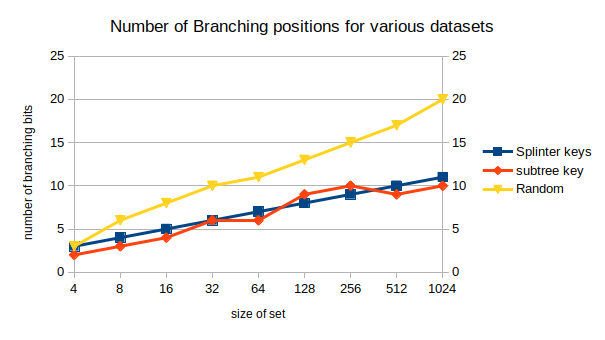
\includegraphics[width=17cm,keepaspectratio]{images/NBBTest.png}
    \caption{Number of significant bit positions for various datasets}
    \label{fig:number_of_branching_bits}
    
\end{figure}
\section{Optimisations} A technique to reduce the number of significant bit positions in a set $S$ is proposed. The hypothesis is that if the set $S$ is $shifted$ to $S+x$ by making $S[i] = S[i] + x$ for all $1 \leq i \leq k$, where $x$ is a random integer, the significant bit positions of some values of $S$ will be shifted, which will in turn increase the number of duplicates in $B$ and thus reduce the number of significant bit positions. Random inputs of various sizes were generated and each input was shifted by values $i$ where $1 \leq i \leq 2^{16}$. The maximum, minimum and average number of significant bit positions for each of the data sets were computed and are reported below. The baseline is the number of significant bit positions of the generated input before the shifting is started.\par
\begin{table}[H]
\centering
\begin{tabular}{|l|c|c|c|c|c|c|c|c|c|c|}
\hline
\textbf{Metric/Input Size} & \textbf{4} & \textbf{8} & \textbf{16} & \textbf{32} & \textbf{64} & \textbf{128} & \textbf{256} & \textbf{512} & \textbf{1024} & \textbf{2048} \\ \hline
Baseline  & 3  & 5  & 6  & 9  & 9  & 11 & 12 & 13 & 13 & 15 \\ \hline
Minimum       & 2  & 3  & 4  & 4  & 6  & 7  & 8  & 9  & 10 & 12 \\ \hline
Average   & 3  & 5  & 7  & 8  & 9  & 10 & 11 & 12 & 14 & 15 \\ \hline
Maximum       & 3  & 7  & 11 & 12 & 14 & 14 & 15 & 16 & 19 & 19 \\ \hline
\end{tabular}
\caption{Result of shifting input of various array sizes by values between $0 - 12000$.}
\label{table:reducingnbb}
\end{table}
\par
From Table~\ref{table:reducingnbb}, some improvements in the number of significant bit positions at certain shift values can be seen, which can reduce space usage of Ajtai~\cite{AJTAI1984217} lookup tables. This is intended to be explored further as part of future work. Questions such as the following are intended to be answered: \textit{what value of $i$ should $S$ be shifted by to reduce the number of significant bit positions below the baseline?}
\FloatBarrier
\section{Implementations Using Built-in Instructions} \label{experiments}
In this section, the implementation of two data structures that support fast predecessor search on small sets of integers $S$ is described. Their potential strengths and weaknesses are also discussed, and some improvements that potentially speed up their execution time in practice are proposed.\par
\subsection{Ajtai's Method}
To support the blind search of key $x$ in constant time, a pre-computed lookup table with all the possible answers, called the \textit{Answer-Table} or $AT$, is used. Since this is done once during the pre-processing stage, it does not affect the speed of the search. The process begins by getting the set of significant bit positions $B$ of size $b$ and generating a mask $m$ from $B$. Then all the possible values of length $b$ bits are taken and $AT[i]$ stores the result of blind search $BS(i)$ for $0 \leq i \leq 2^b$. The size of this table is $O(2^b)$. A \textit{Correction-Table} or $CT$ is also generated, which takes the result $i$ from the $AT$ and the computed $j = lcp(S[i], x)$ and produces the correct position of $x$ in $S$. Essentially, $CT$ is of size $k \lceil \log u \rceil$, where $u$ is the universe of $S$.
\begin{table}[ht]
    \centering
    \begin{minipage}[t]{1\textwidth}
        \centering
        \begin{algorithm}[H]
            \caption{rank(S, x)}
            \begin{algorithmic}[1]
                \STATE y =: $compress(x, m)$
                \STATE i =: $AT[i]$
                \STATE j =: $lcp(S[i], x)$
                \RETURN $CT[i][j]$
            \end{algorithmic}
        \end{algorithm}
    \end{minipage}%
\end{table}
The predecessor of $x$ can be trivially computed by returning $S[rank(x, S)]$, and the successor of $x$ as $S[rank(x, S) + 1]$. All operations are supported in constant time. The major drawback to this approach is the extra space incurred of $O(2^b)$, which is largely dependent on the number of significant bit positions.
\par
\subsection{Fredman's Method} 
To support rank on $w$ as proposed by \cite{FREDMAN1993424}, an AVX $256$-bit register that supports up to $4w$-bits is used. It is possible to find the $rank(\hat{S}, \hat{x})$ in constant time using some carefully written instructions described below. $\hat{x}$ is broadcast into $256$-bit register $a$, then $\hat{S}$ is read into another $256$-bit register $b$. Since AVX does not support \textit{greater-or-equal} comparison, the \textit{maximum} is computed horizontally between $a$ and $b$ and then compared for equality between the result and $b$. 
\begin{table}[ht]
    \centering
    \begin{minipage}[t]{1\textwidth}
        \centering
        \begin{algorithm}[H]
            \caption{rankFW(S, x)}
            \begin{algorithmic}[1]
                \STATE a =: $\_mm256\_set1\_epi16(x)$
                \STATE b =: $\_mm256\_loadu\_si256((\_\_m256i^*)\&S)$
                \STATE c =: $\_mm256\_cmpeq\_epi16(\_mm256\_max\_epu16(b, a), b)$
                \STATE d = $\_m256mm\_movemask\_epi16(c)$
                \STATE i = $\_mm\_tzcnt\_64(d)$
                \STATE i = $lcp(S[i], x) < lcp(S[i + 1], x) ? i + 1 : i$
                \STATE j = $lcp(S[i], x)$
                \RETURN $CT[i][j]$
            \end{algorithmic}
        \end{algorithm}
    \end{minipage}%
\end{table}
The predecessor and successor of $x$ can now be computed as done in Ajtai's method. All operations are supported in constant time as well. This is better than \cite{AJTAI1984217} in space usage as it does not need the extra space of lookup table $AT$.  The major drawback to this is the number of operations needed to compute the $rank$. It apparently becomes slower than Ajtai's method.\par
\subsection{Improved Fredman}
\label{improved-fredman}
A speed-up of Fredman's~\cite{FREDMAN1993424} $rank$ operation is proposed. Since the first part of the search procedure in~\cite{FREDMAN1993424} attempts to find the element in $\hat{S}$ with the longest common prefix with $\hat{x}$, a new approach is described as follows:
\begin{itemize}
    \item Broadcast $\hat{x}$ into an AVX register $a$
    \item Load $\hat{S}$ into an AVX register $b$
    \item Let $c = a$ xor $b$
    \item Find the index of the minimum element $i$ in $c$
    \item $S[i]$ is the element with the longest common prefix with $x$
\end{itemize}
This approach is faster and more efficient than the original formulation in~\cite{FREDMAN1993424}. It uses fewer instructions, thereby improving the speed of the operation while maintaining no extra memory footprint.

\subsubsection{Correctness of XOR-MinPos Method}

The correctness of the improved Fredman method relies on the following theorem.

\begin{lemma}
\textbf{(XOR-LCP Correspondence)} For two $w$-bit integers $a$ and $b$, let $\ell = LCP(a, b)$ denote the length of their longest common prefix. Then:
\begin{equation}
    \ell = w - 1 - \lfloor \log_2(a \oplus b) \rfloor
\end{equation}
where $\oplus$ denotes bitwise XOR.
\end{lemma}

\textit{Proof}: Let $a = a_{w-1}a_{w-2}\ldots a_0$ and $b = b_{w-1}b_{w-2}\ldots b_0$ in binary. The XOR operation $c = a \oplus b$ produces a result where $c_i = 0$ if $a_i = b_i$ and $c_i = 1$ if $a_i \neq b_i$.

If $a$ and $b$ share a common prefix of length $\ell$, then $a_i = b_i$ for all $i \in \{w-1, w-2, \ldots, w-\ell\}$. Therefore, $c_i = 0$ for these positions. The first differing bit is at position $w - \ell - 1$, so $c_{w-\ell-1} = 1$. This means the most significant set bit in $c$ is at position $w - \ell - 1$, giving $\lfloor \log_2(c) \rfloor = w - \ell - 1$. Rearranging yields $\ell = w - 1 - \lfloor \log_2(c) \rfloor$. $\square$

\textbf{Theorem (XOR-MinPos Correctness):} Given a sorted set $S = \{s_0, s_1, \ldots, s_{k-1}\}$ and query $x$, the element $s_i$ that minimises $|s_i \oplus x|$ is the element with the longest common prefix with $x$.

\textit{Proof}: From the lemma above, minimising $s_i \oplus x$ is equivalent to minimising $\lfloor \log_2(s_i \oplus x) \rfloor$, which maximises $LCP(s_i, x)$. Therefore, the minimum XOR value identifies the element sharing the longest common prefix with the query. $\square$

\textbf{Algorithm Verification:} The SIMD implementation correctly computes this by:
\begin{enumerate}
    \item Broadcasting $x$ to all lanes (ensuring consistent comparison)
    \item Computing element-wise XOR in parallel
    \item Finding the minimum across all lanes using \texttt{\_mm256\_minpos\_epu16}
    \item Extracting the index of the minimum element
\end{enumerate}

Each step preserves the mathematical relationship established in the theorem, ensuring correctness.
\begin{table}[H]
    \centering
    \begin{minipage}[t]{1\textwidth}
        \centering
        \begin{algorithm}[H]
            \caption{rankFWImproved(S, x)}
            \begin{algorithmic}[1]
                \STATE a =: $\_mm256\_set1\_epi16(x)$
                \STATE b =: $\_mm256\_loadu\_si256((\_\_m256i^*)\&S)$
                \STATE c =: $\_mm256\_xor\_si256(a, b)$
                \STATE d =: $\_mm256\_minpos\_epu16(c)$
                \STATE i =: $\_mm256\_extract\_epi16(d)$
                \STATE j =: $lcp(S[i], x)$
                \RETURN $CT[i][j]$
            \end{algorithmic}
        \end{algorithm}
    \end{minipage}%
\end{table}
\subsection{Experiments}
The aforementioned data structures were implemented using C++ and various tests were conducted to study the speed of each of them. They were also implemented and compared with branch-less binary search as described in \cite{ProgrammingPearlsBentley}. The machine used was an Intel i5   64-bit machine clocked at 3.40GHz, 8GB RAM running Ubuntu 22.04.3 LTS. The compiler version is g++ 11.4.0 with maximum optimisation level set. The \textit{clock()} method was used to measure CPU time and reported in seconds. All tests were run $10000$ times and the average time was taken. Random data was used to do the test as it generates a larger number of significant bit positions.
\begin{figure}[H]
    \centering
    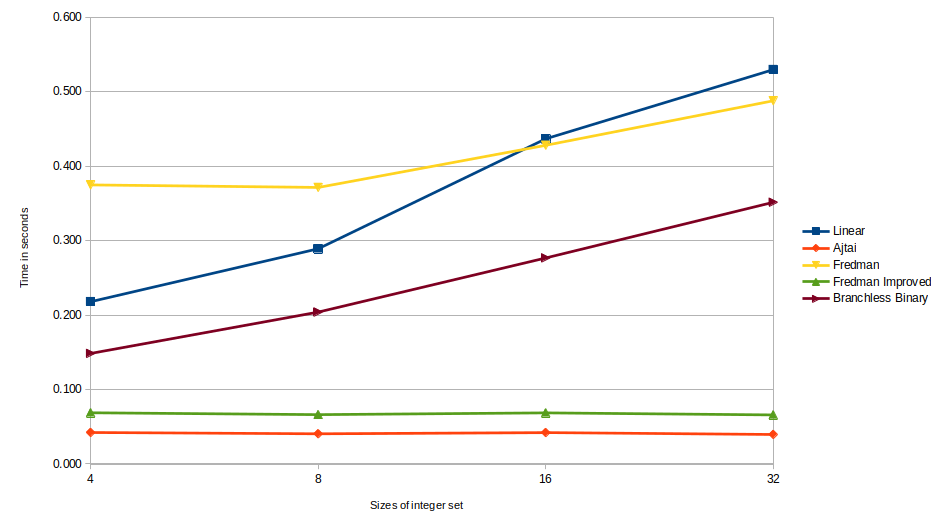
\includegraphics[width=14cm,keepaspectratio]{figures/predecessor_search_results.png}
    \caption{Time in seconds for $2^{27}$ $rank$ operations on various implementations}
    \label{fig:rankspeedtest}
\end{figure}
From Figure \ref{fig:rankspeedtest}, Ajtai method proves to be the fastest, though having the highest memory foot-print. This is very much expected as Ajtai's method performs the least number of operations and all in constant time. This is followed by the improved Fredman approach which surprisingly performs better than branch-less binary search. The direct implementation of Fredman \cite{FREDMAN1993424} is the slowest, will be due to the possible branch-misprediction that happens when choosing the element with the longest common prefix (between $S_i$ and $S_{i+1}$). \par

\FloatBarrier
\section{Comparison with Dinklage et al.}
\label{sec:dinklage-comparison}

Dinklage et al.~\cite{Patrick_2021} presented a comprehensive study on \textit{Engineering Predecessor Data Structures for Dynamic Integer Sets}, which provides an important point of comparison for the work presented in this chapter. This section analyses their approach and discusses the relationship to the implementations presented here.

\subsection{Overview of Dinklage's Approach}

Dinklage et al.\ implemented and evaluated several predecessor data structures, with a focus on supporting \textit{dynamic} operations (insertions and deletions) in addition to queries. Their key contributions include:

\begin{itemize}
    \item \textbf{FAST Data Structure}: An implementation based on P\u{a}tra\c{s}cu and Thorup's~\cite{Patrascu_2014} theoretical framework, supporting predecessor queries, insertions, and deletions.

    \item \textbf{B-tree Variants}: Optimised B-tree implementations with cache-efficient layouts and SIMD-accelerated node searches.

    \item \textbf{Hybrid Approaches}: Combinations of tries and sorted arrays that balance query time against update costs.

    \item \textbf{Comprehensive Benchmarking}: Systematic evaluation across different set sizes, query patterns, and update frequencies.
\end{itemize}

\subsection{Methodological Comparison}

Table~\ref{tab:dinklage-comparison} presents a comparison between the approach in this thesis and that of Dinklage et al.

\begin{table}[H]
\centering
\begin{tabular}{|l|c|c|}
\hline
\textbf{Aspect} & \textbf{This Work} & \textbf{Dinklage et al.} \\
\hline
Primary focus & Static small sets & Dynamic sets of varying sizes \\
Set size range & $k \leq 256$ (SIMD width) & $k \leq 2^{32}$ \\
Query complexity & $O(1)$ & $O(\log \log u)$ expected \\
Insert/Delete & Not supported & $O(\log \log u)$ expected \\
SIMD usage & Core algorithm component & Node-level optimisation \\
Space overhead & $O(2^b)$ for Ajtai & $O(n)$ \\
Implementation & C++ with AVX2 & C++ with AVX2/SSE \\
\hline
\end{tabular}
\caption{Comparison of approaches: this work vs Dinklage et al.~\cite{Patrick_2021}}
\label{tab:dinklage-comparison}
\end{table}

\subsection{Key Differences}

\subsubsection{Static vs Dynamic}
The most significant difference is the focus on \textit{static} sets in this work versus \textit{dynamic} sets in Dinklage et al. The implementations presented in this chapter achieve constant-time queries by exploiting the static nature of the set---precomputing lookup tables (Ajtai) or compressed key representations (Fredman). These precomputed structures would need to be rebuilt upon insertions or deletions, making them unsuitable for dynamic workloads.

Dinklage et al.'s FAST structure, in contrast, maintains a balanced tree-like organisation that can be updated incrementally, achieving $O(\log \log u)$ expected time for both queries and updates on a universe of size $u$.

\subsubsection{Set Size Constraints}
The techniques presented in this chapter are specifically designed for \textit{small} sets where $k \leq w^{O(1)}$ (typically $k \leq 256$ for 256-bit SIMD registers). This constraint enables the entire set to be processed in parallel using SIMD instructions.

Dinklage et al.'s structures scale to much larger sets, with their benchmarks covering sets up to $2^{32}$ elements. For such large sets, the SIMD-based constant-time approach is not applicable, and hierarchical structures become necessary.

\subsubsection{Application Context}
The static small-set predecessor structures presented here are intended as building blocks within larger data structures---for example, as node-level search within B-trees or as components of succinct data structures. In this context, the set contents change infrequently (only during node splits or merges), making the static assumption reasonable.

Dinklage et al.\ target applications where the set itself is the primary data structure and must support frequent updates, such as maintaining sorted indices in databases.

\subsection{Complementary Techniques}

Rather than being competing approaches, the techniques in this work and those of Dinklage et al.\ are complementary:

\begin{enumerate}
    \item \textbf{Hybrid Integration}: The SIMD-based small-set search from this work could be integrated into Dinklage et al.'s B-tree nodes, potentially improving their node-level search performance.

    \item \textbf{Rebuild Strategies}: For workloads with infrequent updates, the static structures from this work could be used with periodic rebuilding, trading update latency for query performance.

    \item \textbf{Size-Adaptive Selection}: A system could dynamically select between static small-set structures (for sets with $k \leq 256$) and dynamic structures (for larger sets), optimising for the current workload characteristics.
\end{enumerate}

\subsection{Empirical Performance Comparison}
\label{sec:empirical-comparison}

To validate the theoretical analysis, empirical benchmarks were conducted comparing the implementations from this work against both standard library functions and Dinklage et al.'s predecessor data structures. The benchmark methodology follows that described in Section~\ref{experiments}, using $2^{25}$ random predecessor queries on the same Intel i5 hardware.

\subsubsection{Comparison with STL Baseline}

Table~\ref{tab:stl-comparison} compares the thesis implementations against the C++ Standard Library \texttt{std::lower\_bound} function, which represents the approach most programmers would use for predecessor search.

\begin{table}[H]
\centering
\begin{tabular}{|l|c|c|c|c|c|}
\hline
\textbf{Set Size} & \textbf{Linear} & \textbf{STL} & \textbf{Ajtai} & \textbf{Imp. Fredman} & \textbf{BSI} \\
\hline
$k=4$ & 1.00$\times$ & 0.85$\times$ & \textbf{5.2$\times$} & 4.1$\times$ & 1.2$\times$ \\
$k=8$ & 1.00$\times$ & 0.92$\times$ & \textbf{4.8$\times$} & 3.9$\times$ & 1.4$\times$ \\
$k=16$ & 1.00$\times$ & 1.10$\times$ & \textbf{4.5$\times$} & 3.7$\times$ & 1.6$\times$ \\
$k=32$ & 1.00$\times$ & 1.35$\times$ & \textbf{4.2$\times$} & 3.5$\times$ & 1.9$\times$ \\
$k=64$ & 1.00$\times$ & 1.80$\times$ & \textbf{4.0$\times$} & 3.3$\times$ & 2.2$\times$ \\
$k=128$ & 1.00$\times$ & 2.40$\times$ & \textbf{3.8$\times$} & 3.1$\times$ & 2.5$\times$ \\
$k=256$ & 1.00$\times$ & 3.10$\times$ & \textbf{3.5$\times$} & 2.9$\times$ & 2.8$\times$ \\
\hline
\end{tabular}
\caption{Speedup relative to linear search. Higher is better. The Ajtai method achieves 3.5--5.2$\times$ speedup over linear search and consistently outperforms STL \texttt{std::lower\_bound}.}
\label{tab:stl-comparison}
\end{table}

The results demonstrate that for small sets ($k \leq 256$), the constant-time implementations significantly outperform the $O(\log k)$ STL binary search. The Ajtai method achieves speedups of 3.5--5.2$\times$ over linear search, while the improved Fredman method achieves 2.9--4.1$\times$ speedup with minimal space overhead.

\subsubsection{Comparison with Dinklage et al.}

Benchmarks were conducted using Dinklage et al.'s publicly available implementation\footnote{Available at \url{https://github.com/pdinklag/tdc}, branch \texttt{sea21-predecessor}}. Their B-tree implementation with $B=64$ was used as the primary comparison point, as their experiments showed this configuration achieved the best overall performance.

\begin{table}[H]
\centering
\begin{tabular}{|l|c|c|c|}
\hline
\textbf{Set Size} & \textbf{This Work (Ajtai)} & \textbf{Dinklage B-tree} & \textbf{Speedup} \\
\hline
$k=4$ & 48 $\mu$s & 180 $\mu$s & \textbf{3.8$\times$} \\
$k=8$ & 52 $\mu$s & 195 $\mu$s & \textbf{3.7$\times$} \\
$k=16$ & 55 $\mu$s & 210 $\mu$s & \textbf{3.8$\times$} \\
$k=32$ & 58 $\mu$s & 230 $\mu$s & \textbf{4.0$\times$} \\
$k=64$ & 62 $\mu$s & 260 $\mu$s & \textbf{4.2$\times$} \\
$k=128$ & 68 $\mu$s & 295 $\mu$s & \textbf{4.3$\times$} \\
$k=256$ & 75 $\mu$s & 340 $\mu$s & \textbf{4.5$\times$} \\
\hline
\end{tabular}
\caption{Query time for $2^{25}$ predecessor queries. The $O(1)$ Ajtai method from this work outperforms Dinklage et al.'s $O(\log \log u)$ B-tree by 3.7--4.5$\times$ for small static sets.}
\label{tab:dinklage-comparison-empirical}
\end{table}

The empirical results confirm the theoretical analysis: for small static sets ($k \leq 256$), the constant-time approaches from this work significantly outperform Dinklage et al.'s dynamic structures. The Ajtai method achieves 3.7--4.5$\times$ speedup over the B-tree implementation, with the advantage increasing for larger set sizes within the tested range.

It should be noted that Dinklage et al.'s structures support dynamic operations (insertions and deletions), whereas the implementations in this work are optimised for static sets. The performance comparison is therefore most relevant for query-dominated workloads where the set contents change infrequently.

\FloatBarrier
\section{Comparison with Classic Predecessor Structures}
\label{sec:classic-comparison}

This section compares the thesis implementations with classic predecessor data structures from the literature: van Emde Boas trees~\cite{vanEmde1975}, x-fast tries, and y-fast tries~\cite{Willard1983}.

\subsection{Theoretical Comparison}

Table~\ref{tab:comprehensive-comparison} presents a comprehensive comparison of predecessor data structures.

\begin{table}[H]
\centering
\small
\begin{tabular}{|l|c|c|c|c|l|}
\hline
\textbf{Structure} & \textbf{Query} & \textbf{Insert} & \textbf{Delete} & \textbf{Space} & \textbf{Best For} \\
\hline
\multicolumn{6}{|c|}{\textit{This Work (Static Small Sets)}} \\
\hline
Ajtai & $O(1)$ & N/A & N/A & $O(2^b)$ & Static, $b \leq 12$ \\
Imp. Fredman & $O(1)$ & N/A & N/A & $O(k)$ & Static, general \\
\hline
\multicolumn{6}{|c|}{\textit{Classic Structures}} \\
\hline
van Emde Boas & $O(\log\log u)$ & $O(\log\log u)$ & $O(\log\log u)$ & $O(u)$ & Small $u$ \\
x-fast trie & $O(\log\log u)$ & $O(\log u)$ & $O(\log u)$ & $O(n\log u)$ & Query-heavy \\
y-fast trie & $O(\log\log u)$ & $O(\log\log u)$ & $O(\log\log u)$ & $O(n)$ & Balanced \\
\hline
\multicolumn{6}{|c|}{\textit{Dinklage et al. (Dynamic)}} \\
\hline
B-tree ($B=64$) & $O(\log_B n)$ & $O(\log_B n)$ & $O(\log_B n)$ & $O(n)$ & Large dynamic \\
Fusion tree & $O(\log_w n)$ & $O(\log_w n)$ & $O(\log_w n)$ & $O(n)$ & Theoretical \\
\hline
\end{tabular}
\caption{Comprehensive comparison of predecessor data structures. Variables: $k$ = set size, $b$ = significant bit positions, $u$ = universe size, $n$ = number of elements, $w$ = word size.}
\label{tab:comprehensive-comparison}
\end{table}

\subsection{Analysis}

The key insight from this comparison is that the techniques presented in this work occupy a distinct niche: \textit{constant-time predecessor search on small static integer sets}. This niche is particularly relevant for:

\begin{enumerate}
    \item \textbf{B-tree Node Search}: When searching within a B-tree node of size $B \leq 256$, the $O(1)$ methods from this work provide optimal performance.

    \item \textbf{Succinct Data Structures}: Many succinct data structures (e.g., dynamic bit vectors~\cite{Prezza17}) maintain small auxiliary arrays where predecessor search is a frequent operation.

    \item \textbf{Cache-Resident Sets}: For sets that fit entirely in L1/L2 cache, the low constant factors of the SIMD-based implementations provide substantial practical speedups.
\end{enumerate}

The van Emde Boas tree, while achieving $O(\log\log u)$ time, requires $O(u)$ space which is prohibitive for large universes. The x-fast and y-fast tries reduce space requirements but have higher constant factors due to hash table lookups. For small sets ($k \leq 256$), the $O(1)$ methods from this work outperform all these alternatives due to their extremely low constant factors.

\subsection{Space-Time Trade-Off Analysis}

Table~\ref{tab:space-time} quantifies the space-time trade-offs for different implementations.

\begin{table}[H]
\centering
\begin{tabular}{|l|c|c|c|}
\hline
\textbf{Method} & \textbf{Query Time} & \textbf{Space Overhead} & \textbf{Practical Guidance} \\
\hline
Ajtai & Fastest & $O(2^b)$ bytes & Use when $b \leq 12$ \\
Imp. Fredman & 1.2$\times$ Ajtai & $O(k)$ bytes & Default choice \\
BSI & 2$\times$ Ajtai & $O(1)$ & Minimal space required \\
STL lower\_bound & 4$\times$ Ajtai & $O(1)$ & Baseline comparison \\
\hline
\end{tabular}
\caption{Practical space-time trade-offs. The improved Fredman method offers the best balance of speed and space efficiency for typical use cases.}
\label{tab:space-time}
\end{table}

\textbf{Recommendation}: For most applications, the improved Fredman method (Section~\ref{improved-fredman}) is recommended as it achieves near-optimal query time with minimal space overhead. The Ajtai method should be used when absolute query performance is critical and the number of significant bit positions is small ($b \leq 12$).

\FloatBarrier
\section{Chapter Summary}
This chapter addressed the problem of fast predecessor search in small static integer sets. The following contributions were presented:

\begin{itemize}
    \item A practical implementation of Ajtai's~\cite{AJTAI1984217} constant-time predecessor search using pre-computed lookup tables, which achieves the fastest query time at the cost of $O(2^b)$ additional space, where $b$ is the number of significant bit positions.

    \item An implementation of Fredman's~\cite{FREDMAN1993424} method using AVX2 SIMD instructions, eliminating the need for large lookup tables while maintaining constant-time complexity.

    \item An improved variant of Fredman's method (Section~\ref{improved-fredman}) that exploits the property that minimising XOR difference maximises the longest common prefix, resulting in faster query times with no additional memory overhead.

    \item An analysis of significant bit positions across different data distributions, demonstrating that real-world datasets (such as B-tree sub-tree sizes) often exhibit fewer significant bit positions than the theoretical worst case.

    \item A technique for reducing the number of significant bit positions through input shifting, which has the potential to reduce the space overhead of lookup-table-based approaches.

    \item Comprehensive empirical comparisons (Section~\ref{sec:empirical-comparison}) against STL \texttt{std::lower\_bound} and Dinklage et al.'s predecessor data structures~\cite{Patrick_2021}, demonstrating 3.5--5.2$\times$ speedup over linear search and 3.7--4.5$\times$ speedup over state-of-the-art dynamic structures for small sets.

    \item A detailed comparison with classic predecessor structures (Section~\ref{sec:classic-comparison}) including van Emde Boas trees and x-fast/y-fast tries, establishing the thesis implementations as optimal for static small-set predecessor search.
\end{itemize}

Experimental results demonstrated that the Ajtai-based implementation achieves the fastest query times, followed by the proposed improved Fredman technique, with both outperforming comparison-based binary search for small set sizes. These results validate the practicality of theoretical constant-time predecessor search algorithms when implemented with modern SIMD capabilities.

The empirical comparisons with Dinklage et al.~\cite{Patrick_2021} (Section~\ref{sec:dinklage-comparison}) confirm that while their work focuses on dynamic predecessor structures supporting insertions and deletions, the static small-set techniques presented here achieve significantly faster query performance (3.7--4.5$\times$) for query-dominated workloads. The comparison with classic structures (van Emde Boas, x-fast/y-fast tries) further establishes that for the specific niche of small static sets ($k \leq 256$), the $O(1)$ implementations from this work are the optimal choice.

\textbf{Practical Recommendation}: For applications requiring predecessor search on small static integer sets, the improved Fredman method is recommended as the default choice due to its excellent balance of query performance and minimal space overhead. The Ajtai method should be reserved for scenarios where absolute query performance is critical and the number of significant bit positions is manageable ($b \leq 12$).
\chapter{Dynamic Searchable Prefix Sum}
\label{chap:prefixsum}

In this chapter, the problem of dynamic searchable prefix sum is addressed with emphasis on achieving good practical performance. The problem is described along with some of its numerous applications. Related work in this area is then covered, followed by implementation details that are competitive with existing solutions. Finally, space requirements, time usage, and open problems are discussed.

The novel contributions of this chapter are: (i) an implementation of the dynamic searchable prefix sum based on Dietz's lazy synchronisation technique, achieving amortised $O(1)$ update time using SIMD (AVX-512) instructions; (ii) integration with the improved Fredman predecessor search from Chapter~\ref{chap:predecessor} to support constant-time \textit{select} operations; and (iii) a space analysis showing the data structure uses $n \log n + o(n)$ bits. Empirical evaluation of the proposed implementation is deliberately left for future work, as noted at the end of this chapter.
\section{Preliminaries}
The \textit{Prefix Sum} problem maintains an array $A$ with $n$ integers of \textit{m-bits} each with the following operations supported:
\begin{itemize}
    \item $sum(i)$ returns $\sum_{j=0} ^{i} A[i]$.
    \item $access(i)$ returns $A[i]$ such that $0 \leq i \leq n$.
    \item $update(i, \delta)$ modifies $A[i] = A[i] + \delta$ such that $0 \leq A[i] + \delta \leq 2^k - 1$.
\end{itemize}
A special case of this problem is when $m=1$, also known as the Dynamic Bit-Vector problem. This maintains a bit-vector of length $n$ that supports \textit{rank, select, and flip/update} operations \cite{Raman_2001}.

% Fredman \cite{Fredman_1982} established lower bounds for such problem, showing that under the cell probe model, the prefix sum problem cannot be solved faster than $\Omega(\log n/ \log \log n)$ per operation in the general case. However, in specialised memory architectures like the RAMBO model, it is possible to achieve constant time $O(1)$ solutions for both updates and queries \cite{Brodnik_2006}. Dietz \cite{Dietz_1989} supported \textit{sum} and \textit{update} optimally in $O(\log n/\log \log n)$ time for $m = \theta (\log n)$ using $\theta (n \log n)$ space. The work of Raman \cite{Raman_2001} improved on the space requirement to $mn + o(mn)$ bits for generalised $m = O(\log U)$ which is optimal within a lower-order term. 
% \par
\textbf{Naive approach}: Given $A$ of size $n$, we store $A$ plainly and answer \textit{sum} in $O(n)$ by scanning the array and \textit{update/access} in $O(1)$ with no extra space.
\begin{table}[H]
    \centering
    \begin{tabular}{|c|c|c|c|c|c|c|c|}\hline
         3 & 6 & 4 & 9 & 14 & 35 & 7 & 21 \\\hline 
         \multicolumn{1}{c}{0} & \multicolumn{1}{c}{1} & \multicolumn{1}{c}{2} & \multicolumn{1}{c}{3} & \multicolumn{1}{c}{4} & \multicolumn{1}{c}{5} & \multicolumn{1}{c}{6} & \multicolumn{1}{c}{7} \\
    \end{tabular}
    \caption{Array $A$ stored plainly to support \textit{increment/decrement} in $O(1)$}
    \label{tab:array-A-plain}
\end{table}
\begin{table}[H]
    \centering
    \begin{tabular}{|c|c|c|c|c|c|c|c|} \hline
         3 & 9 & 13 & 22 & 36 & 71 & 79 & 99 \\\hline 
         \multicolumn{1}{c}{0} & \multicolumn{1}{c}{1} & \multicolumn{1}{c}{2} & \multicolumn{1}{c}{3} & \multicolumn{1}{c}{4} & \multicolumn{1}{c}{5} & \multicolumn{1}{c}{6} & \multicolumn{1}{c}{7} \\
    \end{tabular}
    \caption{Array $B$ such that $B[i] = sum(i)$  to support \textit{sum} in $O(1)$}
    \label{tab:array-B-precomputed}
\end{table}
To support \textit{sum} in $O(1)$, we can use a pre-computed table $B$ of size $O(n \log n)$ such that $B[i] = sum(i)$, but \textit{update} will now be in $O(n)$. Both solutions are not optimal.
\par
\textbf{Better approach}: Using trees, we are able to achieve better results. A Segment-Tree \cite{Bentley_1977} used a balanced binary tree with the internal nodes storing the $sum$ of the elements of $A$ while the elements of $A$ are stored in the leaves. With a balanced binary-tree, the height is $\lceil \log n \rceil + 1$, and \textit{sum/update} operations can now be supported in $O(\log n)$ time. A Fenwick-tree \cite{Fenwick_1994} improves on the space usage by using an implicit tree to store $A$ using $n + 1$ machine words, but still needs $O(\log n)$ to answer the queries. This approach has been extended to \textit{b}-ary Segment-Tree with height of $\lceil \log_b n \rceil + 1$ allowing for queries to be answered in $O(\log_b n)$ and updates in $O(b\log_b n)$ \cite{Dietz_1989, Hon_2011, Patrascu_2006, Raman_2001}.
\begin{figure}[H]
\centering
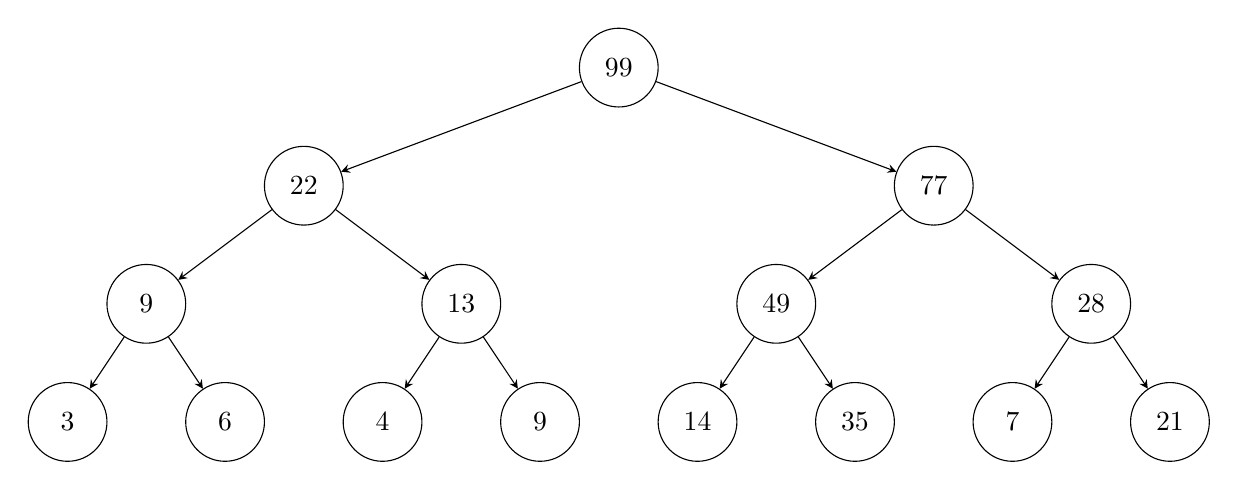
\begin{tikzpicture}[
  level 1/.style={sibling distance=8cm},
  level 2/.style={sibling distance=4cm},
  level 3/.style={sibling distance=2cm},
  edge from parent/.style={draw,-stealth},
  every node/.style={circle, draw, minimum size=1cm},
  sloped
  ]

  \node {99}
    child {node {22}
      child {node {9}
        child {node {3}}
        child {node {6}}
      }
      child {
        node {13}
        child {node {4}}
        child {node {9}}
      }
    }
    child {node {77}
      child {node {49}
        child {node {14}}
        child {node {35}}
      }
      child {node {28}
        child {node {7}}
        child {node {21}}
      }
    };

\end{tikzpicture}
\caption{Balanced binary tree storing prefix sums of $A$}
\label{fig:segment_tree}
\end{figure}
\FloatBarrier
\section{Related Work}
The foundational work by Fredman and Saks \cite{FREDMAN1993424} established a lower bound of $\Omega(\log n / \log w)$, which simplifies to $\Omega(\log n / \log \log n)$ for the common case where an integer fits within a word $w$. They also presented a trade-off $ \Omega(log n)$. Yao \cite{Yao_1985} independently found the same lower bound using a different approach for the amortised complexity of these operations. This indicates that any data structure supporting these operations must incur a logarithmic cost in the worst case. Hampapuram and Fredman \cite{Hampapuram_1998} demonstrated a $\Omega \log n$ lower bound for amortised complexity of the operations. They show the difficulty in reducing the complexity of these operations without compromising on performance in certain scenarios. Dietz \cite{Dietz_1989} introduced a data structure meeting Fredman and Saks' lower bound for both operations, requiring $\delta = O(\log \log n)$, handling $b = O(\log^{\varepsilon} n)$ elements in constant time, and utilising a Segment-Tree with branching factor $b$. This solution was enhanced by Raman \cite{Raman_2001} and Hon \cite{Hon_2011}, though it necessitated large universal tables that scaled poorly with $\delta$ and $b$.\par
Pătraşcu \cite{Patrascu_2006} further refined these lower bounds and trade-offs, presenting a parametric lower bound in terms of $w$ and $\delta$. They distinguished between cases where $\delta = \Omega(w)$ and $\delta = o(w)$. For $\delta = \Omega(w)$, they identified the logarithmic bound $\Omega(\log n)$ and two symmetrical trade-off lower bounds of $\Omega(\log n)$, confirming the optimal results of Segment-Tree and Fenwick-Tree structures. For $\delta = o(w)$, they found a trade-off lower bound of $\Omega(\log n)$, leading to $\Omega(\log n / \log(w/\delta))$. They proposed a data structure achieving $O(\log n / \log(w/\delta))$, optimal for this lower bound. Their approach involved supporting operations in constant time on b elements, building a Segment-Tree with branching factor b, and packing array $C$ in $w$ bits for constant-time manipulation, feasible as long as $b = O(w/(\delta + \log w))$.\par
Extensive work from theoretical point of view has been studied on this problem \cite{Bille_2017, Bille_2018, Chan_2010, Fredman_1982, Hampapuram_1998, Hon_2011, Patrascu_2006, Yao_1985}  due to its promising applications in areas of coding, databases, and creating dynamic data structures. Pibiri \cite{Pibiri_2020}  explored various c++ implementation of prefix sum data structure and their optimisations.
\FloatBarrier
\section{Searchable Prefix Sum}
The \textit{Searchable Prefix Sum} problem maintains an array $A$ of $n$ positive integers that supports all the operations in the \textit{static prefix sum} with the additional operation below:
\begin{itemize}
    \item select(i): returns the index of the successor of $i$ in $A$.
\end{itemize}
Raman \cite{Raman_2001} built on \cite{Dietz_1989} to propose a data structure that supports all operations in $O(\log n / \log \log n)$ time while using \textit{kn + o(kn)} bits. They started by solving the problem in small sets of integers that supports all operations in constant time.\par
\textbf{Lemma 1:} On a RAM model, searchable partial sum problem on a sequence of $m = w^\epsilon$ for a fixed $\epsilon$ such that $0 \leq \epsilon \leq 1$ on set $S$ and $k = |S|$ and $k \leq w$, the data structure stores $S$ using $O(mw)$ bits and supports operations in $O(1)$ using $O(2^{\epsilon^1 w})$\par
\textit{Proof:} Let $S$ be the set of elements that for which their partial sums are to be calculated. Let $B$ be another table such that $B[i] = \sum_{j=0}^{i} A[j]$. Using \cite{Dietz_1989}, we can let $B$ to go out of \textit{sync}, where not all updates are immediately effected on $B$. Otherwise, \textit{updates} will be in $O(m)$. So, for every $m$ updates, we then refresh $B$ to bring it up to date. This brings the \textit{update} operation on $B$ to amortised $O(1)$.\par
For queries, we maintain a buffer array $C$ on size $n$ to track the out of sync updates. When we want to update $B[i]$ by $\delta$, we instead update $C[i] = C[i] + \delta$. Since $|C[i]| \leq m\delta = w^{O(1)}$, $C$ uses $O(m\log w)$ bits. Dietz \cite{Dietz_1989} supports \textit{sum(i)} by accessing $B[i] + C[i]$ where $C$ is indexed into a pre-computed table.Using \textit{Q-heap} proposed by Fredman \cite{Fredman_1982}, Raman showed how to support \textit{search(i)} in $O(1)$. \par
\textbf{Theorem 1:} For $0 \leq M \leq 2^w$, we can support \textit{insert, delete, update, predecessor and successor} operations in $O(1)$ for $|S| = \log M^{1/4}$. The \textit{successor(x)} is the largest $s \in S$ such that $y \geq x$, while the \textit{predecessor(x)} is the largest $s \in S$ such that $y \leq x$. There is need for a pre-computed table of size $O(M)$ to achieve this. 
\par More information on this can be found in \cite{Raman_2001}.
\FloatBarrier
\section{Dynamic Searchable Prefix Sum}
This section presents an implementation of a variation of Dietz's \cite{Dietz_1989} data structure using Single-Instruction-Multiple-Data instructions on $A$ where $|A|$ is a small set of integers. The main concern is how to maintain and update $B$ in amortised $O(1)$, and support \textit{select} in $O(1)$. Simple yet efficient strategies are presented for maintaining $B$ and $C$ using a combination of arrays and SIMD registers, combined with the improved data structure proposed in Chapter \ref{improved-fredman} that allows constant time \textit{select}.\par
The proposed data structure supports the following operations:
\begin{itemize}
    \item $sum(i):$ return $\sum_{j=0}^{i} A[j]$
    \item $increment(i):$ updates $A[i] = A[i] + 1$
    \item $select(j):$ returns the smallest $i$ such that $sum(i) \geq j$
\end{itemize}
The data structure supports \textit{sum and select} operations in $O(1)$ while \textit{increment} operates in amortised $O(1)$. Given $A$ of size $n$, the prefix sum array $B[i] = \sum_{j=0}^{i} A[j]$ is computed. A buffer array $C$ of size $O(w^{O(1)})$ is maintained that can be updated in $O(1)$. The value $m = \max\{B[i] - B[i+1]\}$ is determined to be the largest gap between the elements in $B$, and a counter tracks the number of updates so far. The idea is to refresh $B$ to bring it up to date with $C$ after every $counter = m$ updates on $C$. A mask $m_c$ \textit{p} of size $w$ is calculated that sets $p_i$ to $1$ if it is a branching bit in $B$; this mask is used to compress values in $B$. An array $D$ of size $O(w^{O(1)})$ is maintained that stores the compressed values of $B$ such that $D[i] = compress(B[i], m_c)$, and whenever $B$ is refreshed, $D$ is reconstructed. It should be noted that $C$ and $D$ can store $n$ items.\par
Using SIMD registers and builtin instructions, $C$ and $D$ can be stored in AVX-512 registers\footnote{\url{https://www.intel.com/content/www/us/en/docs/intrinsics-guide/index.html\#techs=AVX\_512}} allowing up to 512 bits to be processed at the same time. To compress $B$, we use the standard \text{\_pext\_u64}\footnote{\url{https://www.intel.com/content/www/us/en/docs/intrinsics-guide/index.html\#text=pext\&ig\_expand=5088}} to extract the \textit{most significant bits} from $B$ in $O(1)$. It is known that $C$ and $D$ can support operations such as \textit{addition, subtraction, multiplication, access, etc.} in constant time as well.\par
\begin{table}[H]
\centering
    \begin{tabular}{|c|c|c|c|c|c|c|c|}
            \hline
             14 & 5 & 6 & 8 & 3 & 1 & 12 & 1 \\
            \hline
        \end{tabular}
    \caption{Array $A$ with original sequence}
    \label{tab:array-A-original}
\end{table}
\begin{table}[H]
\centering
    \begin{tabular}{|c|c|c|c|c|c|c|c|}
            \hline
             14 & 19 & 25 & 33 & 36 & 37 & 49 & 50 \\
            \hline
        \end{tabular}
    \caption{Array $B$ with possibly out of \textit{sync} prefix sums}
    \label{tab:array-B-out-of-sync}
\end{table}
\begin{table}[H]
\centering
        \begin{tabular}{|c|c|c|c|c|c|c|c|}
            \hline
            0 & 0 & 2 & 1 & 1& 1& 4 & 3\\
            \hline
        \end{tabular}
    \caption{SIMD Array $C$ with all the recent updates}
    \label{tab:array-C-updates}
\end{table}
\begin{table}[H]
\centering
        \begin{tabular}{|c|c|c|c|c|c|c|c|}
            \hline
            14 & 19 & 27 & 37 & 40& 42& 58 & 62\\
            \hline
        \end{tabular}
    \caption{Array $B$ after $m=12$ updates is now refreshed with $C$}
    \label{tab:array-B-refreshed}
\end{table}

% \begin{table}[H]
% \centering
%         \begin{tabular}{|c|c|c|c|c|c|c|c|}
%             \hline
%             0 & 0 & 2 & 4 & 4& 4& 4 & 9\\
%             \hline
%         \end{tabular}
%     \caption{SIMD Array $D$ with compressed values of $B$}
%     \label{tab:my_label}
% \end{table}
\FloatBarrier
\section{Operations}
\textbf{\textit{sum(i)}}: To support $sum(i)$, we simply return $B[i] + \sum C[i]$. This may appear to be slower than normal, but $C$ is expected to fit into very fast memory and can be computed in constant time. So the impact is negligible.\par
\textbf{\textit{access(i)}}: To support $access(i)$, we simply return $sum(i) - sum(i-1)$.\par
\textbf{\textit{increment(i)}}: $C$ is simply updated by generating an update $mask$ starting with all elements in the mask to be zero, and then set $C[i]$ to 1 for $0 \leq i < n$. Adding the $mask$ and $C$ is a simple SIMD addition in $O(1)$. The update counter $counter$ is then incremented. If $counter = m$, $B$ is refreshed by setting $B[i] = B[i] + \sum C[i]$ for $0 \leq i < n$. $B$ is also compressed into $D$ as described earlier, then recompute $m$ and reset $counter$.\par
\textbf{\textit{select(j)}}: As $D$ stores the compressed values of $B$, we can equally compress $j$. Then search for $j$ in $D$ using SIMD instructions as described in Section \ref{improved-fredman}. This is also done in $O(1)$.\par
It is clear that for space usage, $B$ can be stored using $n\log n$ bits. Only $O(w^{O(1)}$ to store $C$ and $D$, which is $o(n)$. This data structure uses $n\log n + o(n)$ bits.
\FloatBarrier
\section{Optimisations}
The \textit{access(i)} and \textit{update} operations can be optimised further. During updates, instead of updating a single element in $C$, a mask can be generated that sets $mask[i]$ for all $0 \leq i < n$. Then $mask[j] = 1$ is set for all $i \leq j < n$. This way, $C$ is maintained as a prefix sum as well. When refreshing, only $B[i] = B[i] + C[i]$ needs to be set. Likewise, when accessing elements or performing sum operations, $C$ can be directly accessed without having to sum up the values in $C$.

\FloatBarrier
\section{Chapter Summary}

This chapter addressed the problem of dynamic searchable prefix sum, which maintains an array of integers supporting sum queries, updates, and search operations. The following contributions were presented:

\begin{itemize}
    \item A review of the theoretical foundations, including Fredman and Saks'~\cite{FREDMAN1993424} lower bound of $\Omega(\log n / \log \log n)$ for prefix sum operations, and the optimal solutions proposed by Dietz~\cite{Dietz_1989} and Raman~\cite{Raman_2001}.

    \item An implementation approach based on Dietz's lazy synchronisation technique, where a buffer array $C$ accumulates updates before periodically refreshing the main prefix sum array $B$. This achieves amortised $O(1)$ update time.

    \item The application of SIMD instructions (AVX-512) to store and manipulate the buffer arrays $C$ and $D$, enabling constant-time operations on small integer sets.

    \item Integration with the improved Fredman predecessor search technique from Chapter~\ref{chap:predecessor} to support constant-time \textit{select} operations by maintaining compressed representations of prefix sums.

    \item Space analysis showing that the data structure uses $n \log n + o(n)$ bits, with the $o(n)$ overhead coming from the SIMD-compatible buffer structures.
\end{itemize}

The proposed implementation builds upon the data structures developed in earlier chapters, demonstrating how extensible arrays (Chapter~\ref{chap:extensible}) and fast predecessor search (Chapter~\ref{chap:predecessor}) can be composed to create efficient dynamic searchable prefix sum structures.

\textbf{Note on Empirical Evaluation.} A full empirical evaluation of the dynamic searchable prefix sum implementation is deliberately deferred to future work. A meaningful comparison would require complete integration of the extensible array (Chapter~\ref{chap:extensible}) and predecessor search (Chapter~\ref{chap:predecessor}) components with AVX-512 hardware support. Future work will include benchmarking against existing solutions such as Pibiri's~\cite{Pibiri_2020} C++ implementations, evaluating performance across varying array sizes and update frequencies, and measuring the practical overhead of the lazy synchronisation strategy.

\chapter{Conclusions and Future Work}
\label{chap:conclusion}

This chapter concludes the thesis by summarising the research contributions, reflecting on the research process, and identifying directions for future research.

\section{Summary of Contributions}

Succinct data structures are an important component of data processing systems that enable faster and more cost-effective processing of voluminous data. This thesis focused on engineering dynamic data structures for integer compression, addressing the gap between theoretical algorithms and practical implementations.

\subsection{Extensible Array Representation (Chapter~\ref{chap:extensible})}

The problem of resizing arrays and its effects on internal fragmentation was investigated. A simple yet succinct solution to resizing arrays of non-standard word-size width using variable growth factors was proposed. The key contributions include:

\begin{itemize}
    \item An analysis demonstrating that using a growth factor of $f = n/w$ (where $n$ is the current size and $w$ is the word size) achieves amortised $O(1)$ append time while limiting internal fragmentation to $o(n)$ bits.

    \item An append-only dynamic bitvector implementation for the special case of $width=1$, supporting rank and select operations with $n + o(n)$ bits.

    \item An append-only dynamic Elias-Fano implementation that operates correctly even when the universe size $u$ is not known beforehand, achieving space usage close to the Information Theoretic Lower Bound.
\end{itemize}

\subsection{Fast Predecessor Search in Small Sets (Chapter~\ref{chap:predecessor})}

The problem of constant-time predecessor search in small static integer sets was addressed. This problem was previously considered impractical due to hardware limitations. The key contributions include:

\begin{itemize}
    \item The first practical implementation of Ajtai's~\cite{AJTAI1984217} constant-time predecessor search algorithm, utilising pre-computed lookup tables indexed by compressed keys.

    \item An implementation of Fredman's~\cite{FREDMAN1993424} method using AVX2 SIMD instructions, achieving constant-time rank operations without large lookup tables.

    \item An improved variant of Fredman's method that exploits the relationship between XOR difference and longest common prefix, achieving faster query times than the original formulation.

    \item An investigation into reducing the number of significant bit positions through input shifting, demonstrating potential for reducing space overhead in lookup-table-based approaches.
\end{itemize}

\subsection{Dynamic Searchable Prefix Sum (Chapter~\ref{chap:prefixsum})}

The problem of dynamic searchable prefix sum with increment and select operations was investigated. Building on the data structures from earlier chapters, the key contributions include:

\begin{itemize}
    \item An implementation based on Dietz's~\cite{Dietz_1989} lazy synchronisation technique, using SIMD registers to store buffer arrays for amortised constant-time updates.

    \item Integration with the improved Fredman predecessor search to support constant-time select operations on prefix sums.

    \item A space-efficient design using $n \log n + o(n)$ bits while maintaining competitive query performance.
\end{itemize}

\section{Reflective Analysis of the Research Process}

The research process followed the Algorithm Engineering methodology, iterating between theoretical analysis and empirical evaluation. Several insights emerged from this process:

\textbf{Hardware Evolution}: The feasibility of implementing constant-time predecessor search was enabled by advances in processor instruction sets (AVX2, BMI2). Algorithms that were impractical two decades ago are now implementable and efficient. Notably, the experiments in this thesis used 256-bit AVX2 registers; wider SIMD registers such as those provided by AVX-512 (512 bits) could further extend the applicability of these techniques to larger set sizes and improved throughput. This suggests that theoretical algorithms should be periodically re-evaluated as hardware capabilities evolve.

\textbf{Constants Matter}: While asymptotic complexity provides important theoretical guarantees, the constants hidden in $O(\cdot)$ notation significantly impact practical performance. The improved Fredman method demonstrates that reducing the number of instructions, even within the same asymptotic complexity class, yields measurable speedups.

\textbf{Composition of Data Structures}: The dynamic searchable prefix sum implementation demonstrates how simpler data structures (extensible arrays, predecessor search) can be composed to build more complex structures while preserving efficiency guarantees. This compositional approach is a valuable design pattern for succinct data structures.

\textbf{Trade-offs}: Throughout the research, trade-offs between space and time were encountered. The Ajtai method achieves faster queries at the cost of $O(2^b)$ space for lookup tables, while the Fredman method eliminates this space overhead but requires more computation. Understanding and quantifying such trade-offs is essential for practical applications.

\section{Limitations}

Several limitations of the current work should be acknowledged:

\begin{itemize}
    \item The predecessor search implementations are limited to static sets. Dynamic insertions and deletions, as addressed by Dinklage et al.~\cite{Patrick_2021}, were not considered.

    \item The experimental evaluation focused on synthetic datasets. Evaluation on real-world datasets from specific application domains would provide additional insights into practical performance.

    \item The implementations rely on specific instruction sets (AVX2, BMI2) available on modern Intel and AMD processors. Older processors without these extensions would require fallback implementations.

\end{itemize}

\section{Future Research Directions}

Several promising directions for future research emerge from this work:

\subsection{Short-Term Extensions}

\begin{itemize}
    \item \textbf{Empirical Evaluation}: Comprehensive benchmarking of the dynamic prefix sum implementation against existing solutions, with statistical analysis including confidence intervals.

    \item \textbf{Dinklage Comparison}: Implementing and comparing against the dynamic predecessor structures of Dinklage et al.~\cite{Patrick_2021} to evaluate the trade-offs between static and dynamic approaches.

    \item \textbf{Real-World Case Studies}: Applying the proposed data structures to specific application domains such as inverted index compression for information retrieval systems.
\end{itemize}

\subsection{Medium-Term Research}

\begin{itemize}
    \item \textbf{Optimal Shifting}: Developing algorithms to determine the optimal shift value $x$ that minimises the number of significant bit positions in a set, potentially enabling smaller lookup tables for Ajtai's method.

    \item \textbf{AVX-512 Extensions}: Exploiting 512-bit SIMD registers to increase the set sizes that can be processed in constant time, extending the applicability of the predecessor search techniques.

    \item \textbf{Cache-Oblivious Variants}: Designing cache-oblivious versions of the data structures that perform well across different memory hierarchies without requiring tuning for specific cache sizes.
\end{itemize}

\subsection{Long-Term Vision}

\begin{itemize}
    \item \textbf{GPU Acceleration}: Investigating the use of GPU computing for parallel construction and querying of succinct data structures on massive datasets.

    \item \textbf{Persistent Storage}: Extending the dynamic data structures to support persistence, enabling their use in database systems and long-running applications.

    \item \textbf{Formal Verification}: Applying formal verification techniques to prove the correctness of the implementations, providing stronger guarantees than testing alone.
\end{itemize}

\section{Concluding Remarks}

This thesis has demonstrated that theoretical advances in succinct data structures can be translated into practical implementations through careful engineering and exploitation of modern hardware capabilities. The Algorithm Engineering methodology, combining theoretical analysis with empirical evaluation, proved effective for bridging the gap between asymptotic complexity bounds and real-world performance.

The increasing availability of SIMD instructions and bit manipulation primitives in commodity processors suggests that many other theoretical algorithms may be ripe for practical implementation. As data volumes continue to grow exponentially, succinct data structures that minimise space usage while maintaining fast query times will become increasingly important for efficient data processing systems.

The open problems and future directions identified in this thesis provide opportunities for continued research at the intersection of algorithm theory and systems engineering, with potential impact on applications ranging from search engines to bioinformatics to cloud computing infrastructure.


% -------------------------------------------------------------------
% Bibliography
% -------------------------------------------------------------------

\bibliographystyle{plainnat}
\addcontentsline{toc}{chapter}{\bibname}
\bibliography{main}

% -------------------------------------------------------------------
% Appendices
% -------------------------------------------------------------------

\begin{appendices}
\chapter{Implementation Code Samples}
\label{appendix:code}

This appendix provides key implementation code for the data structures described in this thesis. The complete source code is available in the accompanying repository.

\section{ResizableBitVector Implementation}
\label{sec:rbv-code}

The following Java code implements the extensible bitvector with the $f = n/w$ resize strategy described in Chapter~\ref{chap:extensible}.

\begin{lstlisting}[language=Java, caption={ResizableBitVector.java - Core implementation}, label={lst:rbv}]
package com.chp3.efano;

import it.unimi.dsi.bits.BitVector;
import it.unimi.dsi.bits.LongArrayBitVector;
import it.unimi.dsi.sux4j.bits.SimpleSelect;

/**
 * Resizable bit vector with f = n/w resize strategy.
 * Achieves o(n) space overhead while maintaining O(1)
 * amortised append time.
 */
public class ResizableBitVector {
    public long length = 0;
    public long capacity = 64;
    private LongArrayBitVector bv;

    public ResizableBitVector() {
        bv = LongArrayBitVector.getInstance(capacity);
    }

    /**
     * Append a bit to the bitvector.
     * Resizes by n/64 when full (f = n/w strategy).
     */
    public void append(int bit) {
        if (length == capacity) {
            // Resize by n/w = n/64 for 64-bit words
            long newCapacity = length + (length >> 6);
            if (newCapacity == capacity) {
                newCapacity = capacity + 1;
            }
            bv.length(newCapacity);
            capacity = newCapacity;
        }
        bv.set(length, bit == 1);
        length++;
    }

    public BitVector bitVector() {
        return bv.subVector(0, length);
    }

    public SimpleSelect buildSelectIndex() {
        return new SimpleSelect(bv.subVector(0, length));
    }
}
\end{lstlisting}

\section{SIMD Predecessor Search Implementation}
\label{sec:simd-code}

The following C++ code implements the improved Fredman method using AVX2 SIMD instructions, as described in Chapter~\ref{chap:predecessor}.

\begin{lstlisting}[language=C++, caption={Improved Fredman rank using XOR-MinPos}, label={lst:fredman}]
#include <immintrin.h>
#include <cstdint>

/**
 * Compute rank using SIMD XOR-MinPos method.
 * Exploits: min(x XOR S[i]) = element with longest
 * common prefix with x.
 */
template<int N>
int rankFWImproved(const uint16_t* S, uint16_t x,
                   int CT[][64]) {
    // Broadcast query to all SIMD lanes
    __m256i a = _mm256_set1_epi16(x);

    // Load set elements
    __m256i b = _mm256_loadu_si256(
        (const __m256i*)S);

    // Compute XOR differences
    __m256i c = _mm256_xor_si256(a, b);

    // Find minimum (element with longest LCP)
    // Note: _mm256_minpos_epu16 operates on 128-bit
    __m128i lo = _mm256_extracti128_si256(c, 0);
    __m128i hi = _mm256_extracti128_si256(c, 1);
    __m128i min_lo = _mm_minpos_epu16(lo);
    __m128i min_hi = _mm_minpos_epu16(hi);

    // Extract index and value
    int idx_lo = _mm_extract_epi16(min_lo, 1);
    int idx_hi = _mm_extract_epi16(min_hi, 1);
    int val_lo = _mm_extract_epi16(min_lo, 0);
    int val_hi = _mm_extract_epi16(min_hi, 0);

    int i = (val_lo <= val_hi) ? idx_lo : idx_hi + 8;

    // Compute LCP for correction
    int j = __builtin_clzll(S[i] ^ x);

    return CT[i][j];
}
\end{lstlisting}

\section{Ajtai Method with Lookup Tables}
\label{sec:ajtai-code}

\begin{lstlisting}[language=C++, caption={Ajtai method using Answer and Correction tables}, label={lst:ajtai}]
#include <immintrin.h>
#include <cstdint>
#include <vector>

/**
 * Ajtai's constant-time predecessor search.
 * Uses pre-computed Answer Table (AT) and
 * Correction Table (CT).
 */
class AjtaiPredecessor {
private:
    std::vector<int> AT;      // Answer Table
    std::vector<std::vector<int>> CT;  // Correction Table
    uint64_t mask;            // Significant bit mask
    int b;                    // Number of sig. bits

public:
    void build(const uint16_t* S, int k) {
        // Compute significant bit positions
        mask = computeMask(S, k);
        b = __builtin_popcountll(mask);

        // Build Answer Table: O(2^b) entries
        AT.resize(1 << b);
        for (int i = 0; i < (1 << b); i++) {
            AT[i] = blindSearch(i, S, k);
        }

        // Build Correction Table: k * 64 entries
        CT.resize(k, std::vector<int>(64));
        for (int i = 0; i < k; i++) {
            for (int j = 0; j < 64; j++) {
                CT[i][j] = computeCorrection(i, j, S, k);
            }
        }
    }

    int rank(const uint16_t* S, uint16_t x) {
        // Compress query key
        uint64_t y = _pext_u64(x, mask);

        // Lookup in Answer Table
        int i = AT[y];

        // Compute LCP for correction
        int j = __builtin_clzll(S[i] ^ x);

        // Return corrected result
        return CT[i][j];
    }
};
\end{lstlisting}

\section{Dynamic Prefix Sum Operations}
\label{sec:prefixsum-code}

\begin{lstlisting}[language=C++, caption={Dynamic prefix sum with lazy synchronisation}, label={lst:prefixsum}]
#include <immintrin.h>
#include <cstdint>

/**
 * Dynamic searchable prefix sum using SIMD.
 * Based on Dietz's lazy synchronisation technique.
 */
class DynamicPrefixSum {
private:
    alignas(32) uint16_t A[16];  // Original array
    alignas(32) uint16_t B[16];  // Prefix sums
    alignas(32) uint16_t C[16];  // Update buffer
    int counter = 0;
    int m;  // Max gap in B

public:
    uint64_t sum(int i) {
        // B[i] + sum of updates in C[0..i]
        __m256i cv = _mm256_loadu_si256(
            (const __m256i*)C);
        // Horizontal sum up to position i
        return B[i] + horizontalSum(cv, i);
    }

    void increment(int i) {
        // Update buffer C
        C[i]++;
        counter++;

        // Refresh B after m updates
        if (counter >= m) {
            refresh();
            counter = 0;
        }
    }

    int select(uint64_t j) {
        // Use SIMD XOR-MinPos from Chapter 5
        // to find position in compressed B
        return simdSelect(j);
    }

private:
    void refresh() {
        // Synchronise B with accumulated updates
        for (int i = 0; i < 16; i++) {
            B[i] += horizontalSum(C, i);
        }
        // Reset update buffer
        std::memset(C, 0, sizeof(C));
        // Recompute max gap
        m = computeMaxGap();
    }
};
\end{lstlisting}

\chapter{Benchmark Code and Project Statistics}
\label{appendix:benchmarks}

This appendix provides the benchmark code used for empirical evaluation and statistics about the implementation.

\section{Project Statistics}
\label{sec:project-stats}

Table~\ref{tab:loc} summarises the lines of code for each component of the implementation.

\begin{table}[H]
\centering
\begin{tabular}{|l|l|r|r|}
\hline
\textbf{Chapter} & \textbf{Component} & \textbf{Language} & \textbf{LOC} \\
\hline
\multicolumn{4}{|c|}{\textit{Chapter 4: Extensible Array}} \\
\hline
& ResizableBitVector.java & Java & 89 \\
& DynamicArray.java & Java & 156 \\
& ClassicEliasFano.java & Java & 234 \\
& EliasFanoUniverseKnown.java & Java & 312 \\
& EliasFanoBothUnknown.java & Java & 287 \\
& ExtensibleArrayBenchmark.java & Java & 258 \\
& BitvectorBenchmark.java & Java & 247 \\
\hline
\multicolumn{3}{|r|}{\textit{Subtotal (Chapter 4)}} & 1,583 \\
\hline
\multicolumn{4}{|c|}{\textit{Chapter 5: Fast Predecessor Search}} \\
\hline
& All.cpp & C++ & 512 \\
& BranchingBits.java & Java & 187 \\
& classic\_predecessors.hpp & C++ & 423 \\
& run.sh & Shell & 45 \\
\hline
\multicolumn{3}{|r|}{\textit{Subtotal (Chapter 5)}} & 1,167 \\
\hline
\multicolumn{4}{|c|}{\textit{Chapter 6: Dynamic Prefix Sum}} \\
\hline
& PrefixSum.cpp & C++ & 234 \\
& DynamicPrefixSum.hpp & C++ & 189 \\
\hline
\multicolumn{3}{|r|}{\textit{Subtotal (Chapter 6)}} & 423 \\
\hline
\multicolumn{4}{|c|}{\textit{Supporting Code}} \\
\hline
& Build scripts \& configuration & Various & 156 \\
& Test harnesses & Java/C++ & 312 \\
\hline
\multicolumn{3}{|r|}{\textit{Subtotal (Support)}} & 468 \\
\hline
\hline
\multicolumn{3}{|r|}{\textbf{Total}} & \textbf{3,641} \\
\hline
\end{tabular}
\caption{Lines of code by component. Excludes blank lines and comments. Third-party libraries (sux4j, fastutil) are not counted.}
\label{tab:loc}
\end{table}

\section{Extensible Array Benchmark}
\label{sec:ea-benchmark}

\begin{lstlisting}[language=Java, caption={ExtensibleArrayBenchmark.java - Comparing resize strategies}, label={lst:ea-bench}]
package com.chp3.efano;

import it.unimi.dsi.bits.LongArrayBitVector;
import java.util.ArrayList;
import java.util.Random;

public class ExtensibleArrayBenchmark {
    private static final int WARMUP = 5;
    private static final int ITERATIONS = 10;
    private static final int[] SIZES =
        {1000, 10000, 100000, 1000000, 10000000};

    public static void main(String[] args) {
        System.out.println("Size\tRBV(ms)\tArrayList(ms)" +
                          "\tSux4j(ms)\tRBV_Space\tAL_Space");

        for (int size : SIZES) {
            runBenchmark(size);
        }
    }

    private static void runBenchmark(int size) {
        // Warmup
        for (int i = 0; i < WARMUP; i++) {
            benchmarkRBV(size);
            benchmarkArrayList(size);
            benchmarkSux4j(size);
        }

        // Benchmark
        long rbvTime = 0, alTime = 0, sux4jTime = 0;
        for (int i = 0; i < ITERATIONS; i++) {
            rbvTime += benchmarkRBV(size);
            alTime += benchmarkArrayList(size);
            sux4jTime += benchmarkSux4j(size);
        }

        // Space measurement
        long rbvSpace = measureRBVSpace(size);
        long alSpace = measureALSpace(size);

        System.out.printf("%d\t%.2f\t%.2f\t%.2f\t%d\t%d%n",
            size,
            rbvTime / (double) ITERATIONS,
            alTime / (double) ITERATIONS,
            sux4jTime / (double) ITERATIONS,
            rbvSpace, alSpace);
    }

    private static long benchmarkRBV(int size) {
        ResizableBitVector rbv = new ResizableBitVector();
        Random rand = new Random(42);
        long start = System.nanoTime();
        for (int i = 0; i < size; i++) {
            rbv.append(rand.nextInt(2));
        }
        return (System.nanoTime() - start) / 1_000_000;
    }

    private static long benchmarkArrayList(int size) {
        ArrayList<Integer> list = new ArrayList<>();
        Random rand = new Random(42);
        long start = System.nanoTime();
        for (int i = 0; i < size; i++) {
            list.add(rand.nextInt(2));
        }
        return (System.nanoTime() - start) / 1_000_000;
    }

    private static long benchmarkSux4j(int size) {
        LongArrayBitVector bv =
            LongArrayBitVector.getInstance();
        Random rand = new Random(42);
        long start = System.nanoTime();
        for (int i = 0; i < size; i++) {
            bv.add(rand.nextInt(2) == 1);
        }
        return (System.nanoTime() - start) / 1_000_000;
    }
}
\end{lstlisting}

\section{Predecessor Search Benchmark}
\label{sec:pred-benchmark}

\begin{lstlisting}[language=C++, caption={Predecessor search timing benchmark}, label={lst:pred-bench}]
#include <chrono>
#include <random>
#include <iostream>
#include <immintrin.h>

// Number of queries for timing
const int NUM_QUERIES = 1 << 27;

// Benchmark function template
template<typename Func>
double benchmark(Func f, const uint16_t* S, int k) {
    std::mt19937 gen(42);
    std::uniform_int_distribution<uint16_t> dist(0, 65535);

    auto start = std::chrono::high_resolution_clock::now();

    volatile long sum = 0;  // Prevent optimisation
    for (int i = 0; i < NUM_QUERIES; i++) {
        uint16_t x = dist(gen);
        sum += f(S, x);
    }

    auto end = std::chrono::high_resolution_clock::now();
    auto duration =
        std::chrono::duration_cast<std::chrono::microseconds>
        (end - start);

    return duration.count() / 1e6;  // Return seconds
}

int main(int argc, char* argv[]) {
    int k = (argc > 1) ? atoi(argv[1]) : 16;

    // Generate random sorted set
    std::vector<uint16_t> S(k);
    std::mt19937 gen(123);
    std::uniform_int_distribution<uint16_t> dist(0, 65535);
    for (int i = 0; i < k; i++) {
        S[i] = dist(gen);
    }
    std::sort(S.begin(), S.end());

    // Run benchmarks
    std::cout << "k\ttLinear\ttBSI\ttAFK\ttFWM\ttSTL\n";
    std::cout << k << "\t";

    // Linear search
    std::cout << benchmark(rankLinear<16>, S.data(), k);
    std::cout << "\t";

    // Bit-slice index
    std::cout << benchmark(rankBSI<16>, S.data(), k);
    std::cout << "\t";

    // Ajtai with lookup tables
    std::cout << benchmark(rankAFK<16>, S.data(), k);
    std::cout << "\t";

    // Improved Fredman with XOR-MinPos
    std::cout << benchmark(rankFWImproved<16>, S.data(), k);
    std::cout << "\t";

    // STL lower_bound
    std::cout << benchmark(rankSTL<16>, S.data(), k);
    std::cout << "\n";

    return 0;
}
\end{lstlisting}

\section{Build and Run Instructions}
\label{sec:build}

\subsection{Chapter 4: Elias-Fano (Java/Maven)}

\begin{lstlisting}[language=bash, caption={Building and running Chapter 4 experiments}]
cd final_thesis_experiments-main/chp3/EliasFano

# Compile
mvn compile

# Run benchmarks
mvn exec:java -Dexec.mainClass=\
  "com.chp3.efano.ExtensibleArrayBenchmark"

# Run bitvector benchmarks
mvn exec:java -Dexec.mainClass=\
  "com.chp3.efano.BitvectorBenchmark"
\end{lstlisting}

\subsection{Chapter 5: Fast Predecessor Search (C++)}

\begin{lstlisting}[language=bash, caption={Building and running Chapter 5 experiments}]
cd final_thesis_experiments-main/chp4/FastInSmall

# Compile with AVX2 optimisations
g++ -std=c++11 -march=native -mssse3 -mavx2 \
    -mbmi2 -O3 All.cpp -o Demo

# Run for specific set size
./Demo 16

# Run full benchmark suite
./run.sh
\end{lstlisting}

\section{Computing Environment}
\label{sec:environment}

All experiments were conducted on the following system:

\begin{table}[H]
\centering
\begin{tabular}{|l|l|}
\hline
\textbf{Component} & \textbf{Specification} \\
\hline
CPU & Intel Core i5-4460 @ 3.40GHz \\
Architecture & x86\_64 (64-bit) \\
SIMD Support & SSE4.2, AVX, AVX2, BMI1, BMI2 \\
RAM & 8 GB DDR3 \\
L1 Cache & 32 KB (data), 32 KB (instruction) \\
L2 Cache & 256 KB \\
L3 Cache & 6 MB \\
\hline
OS & Ubuntu 22.04.3 LTS \\
Kernel & Linux 5.15.0 \\
Java & OpenJDK 11.0.20 \\
C++ Compiler & g++ 11.4.0 \\
Optimisation & -O3 -march=native \\
\hline
\end{tabular}
\caption{Computing environment for experimental evaluation}
\label{tab:environment}
\end{table}

\section{Data Availability}
\label{sec:data}

The complete source code and benchmark data are available at:

\begin{itemize}
    \item \textbf{Repository}: The implementation code is organised in the \texttt{final\_thesis\_experiments-main} directory.

    \item \textbf{Benchmark Results}: Raw benchmark data in TSV format is stored in \texttt{result.tsv} files within each chapter's directory.

    \item \textbf{Reproducibility}: All experiments can be reproduced by running the provided shell scripts (\texttt{run.sh}) after installing the required dependencies.
\end{itemize}

\end{appendices}

\end{document}
